\chapter{Mengenal APEX Oracle}

\section{Agenda Kegiatan}
\subsection{Pengembangan Aplikasi dengan Low Code}
Apa yang dimaksud dengan Low Code?\\
Low Code merupakan pengembangan aplikasi berbasis GUI, sehingga memungkinkan untuk mengembangkan sebuah aplikasi tanpa perlu menuliskan baris kode yang banyak.\\
\begin{enumerate}
 \item Low code mudah untuk dijalankan karena kita hanya membutuhkan data-data, parameter, dan gambaran dari aplikasi yang akan kita buat. Setelah pembuatan aplikasi berhasil, kita hanya perlu mengklik tombol Jalankan Aplikasi pada GUI yang tampil.
 \item Sangat produktif karena aplikasi berbasis low code telah menyediakan banyak fitur yang bisa kita tambahkan pada aplikasi yang ingin kita buat dan telah berbasis GUI.
 \item Nyata karena setelah pembuatan aplikasi selesai kita dapat  menggunakan aplikasi tersebut saat itu juga, kita juga tidak membutuhkan waktu lama dalam pembuatan aplikasi.
 \item Dapat diperbaharui, hal ini mempermudah kita dalam melakukan maintenance aplikasi.
 \item kaya akan fungsionalitas dari kode yang sedikit. Dengan kode yang sedikit, memungkinkan untuk membuat dan mengembangkan sebuah program aplikasi, hal ini tentunya merupakan suatu hal yang sangat bagus. Aplikasi yang dibuat dengan Low Code akan meminimalisir biaya yang akan dikeluarkan dalam pembuatan aplikasi.
\end{enumerate}
Platform pengembangan low code memungkinkan developer membangun aplikasi perusahaan yang dapat diskalakan dan aman dengan fitur kelas dunia yang dapat digunakan.\\
Data low code pengembangan aplikasi pertama.
\begin{figure}[H]
    \centering
    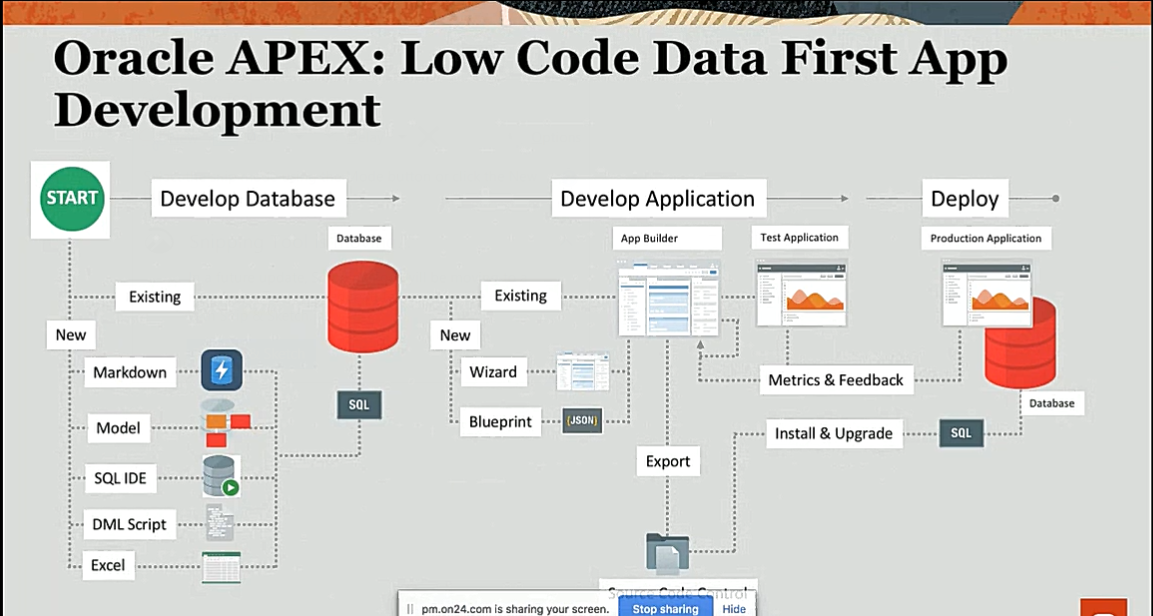
\includegraphics[scale=0.5]{figures/1}
    \caption{\textit{First App APEX}}
    \label{FirstApp}
\end{figure} 

\subsection{Penjelasan Mengenai Oracle Application Express}
Apa itu oracle Apex?\\
Apex merupakan kerangka kerja pengembangan aplikasi web dan database pusat.\\
Fungsi dan Kegunaan APEX:
\begin{enumerate}
 \item Membangun aplikasi desktop dan mobile web app.
 \item Memvisualiasasikan dan memelihata data pada Database.
 \item Meningkatkan kemampuan SQL dan kemampuan basis data.
\end{enumerate}

\subsection{Mengubah Spreadsheet Menjadi Web App dalam Hitungan Menit}
Mengelola data didalam sebuah spreadsheet adalah sebuah tantangan. Ketika mengelola data, harus memperhatikan validasi data. Memperhatikan Integritas Data, karena integritas data tidak dapat menjamin keakuratan data dalam lingkungan multiuser. Memperhatikan Keamanan data. Berhati-hati saat melakukan data sharing, karena spreadsheet bersifat easy to share.\\
Berikut langkah-langkah Mengubah Spreadsheet menjadi Web App:
\begin{enumerate}
 \item Login APEX, masukkan workspace, username, dan password APEX.
 \begin{figure}[H]
    \centering
    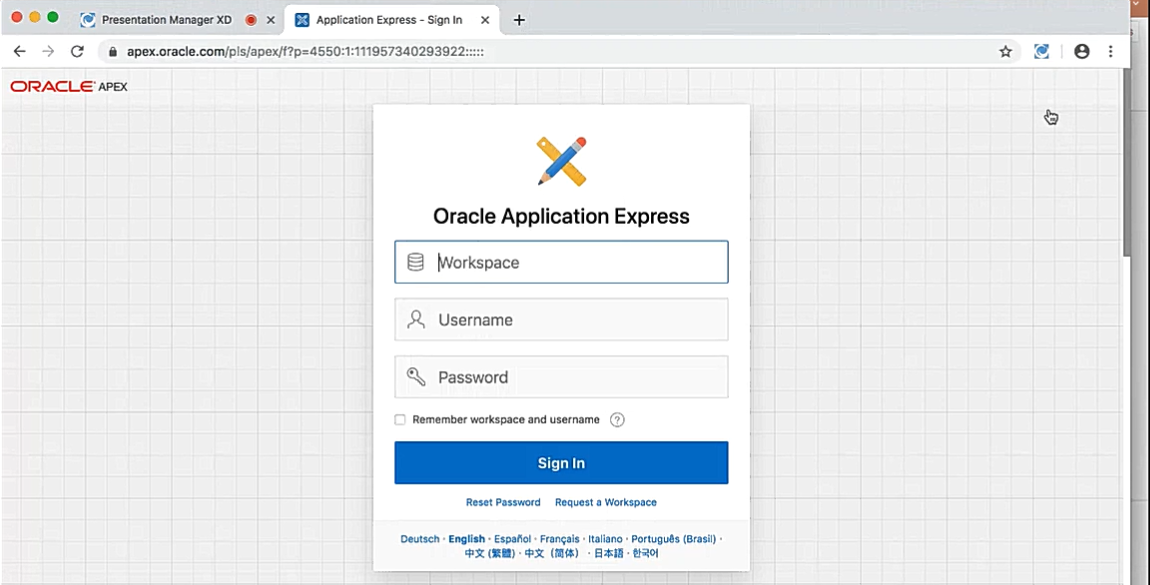
\includegraphics[scale=0.5]{figures/2}
    \caption{\textit{Login}}
    \label{Login}
\end{figure}
 \item Pilih menu App Builder.
 \begin{figure}[H]
    \centering
    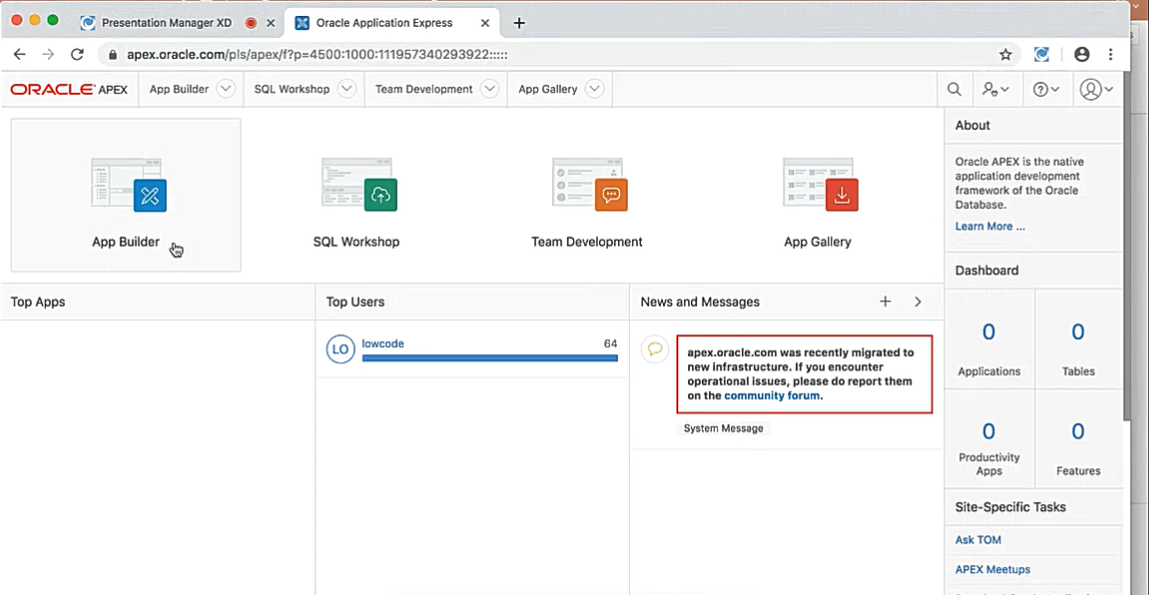
\includegraphics[scale=0.5]{figures/3}
    \caption{\textit{App Builder}}
    \label{AppBuild}
\end{figure}
 \item Pilih menu Create.
 \begin{figure}[H]
    \centering
    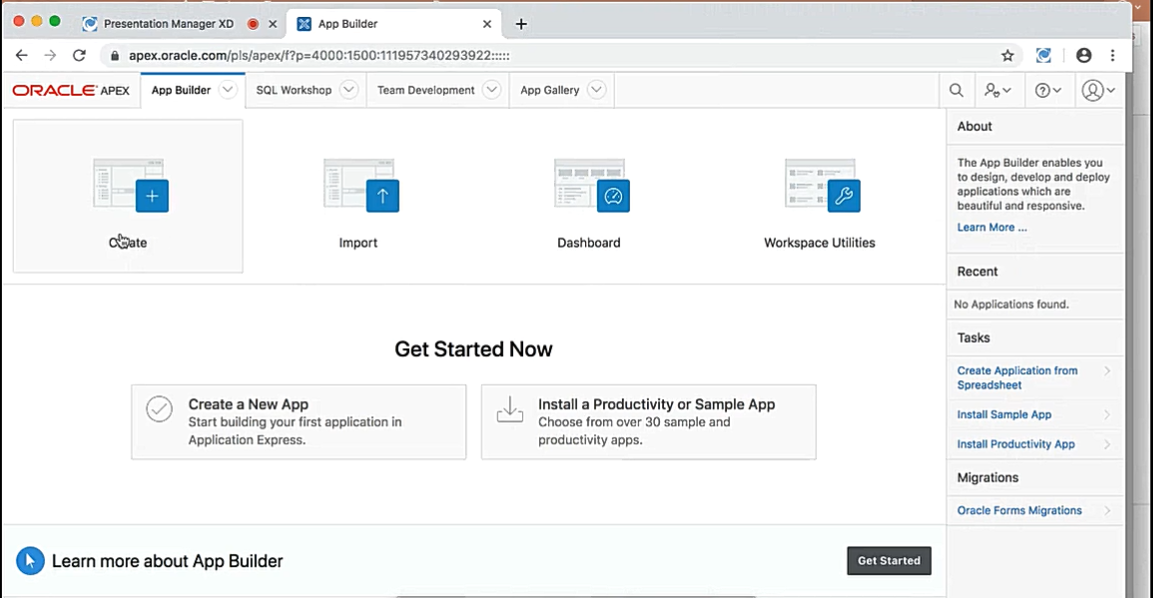
\includegraphics[scale=0.5]{figures/4}
    \caption{\textit{Create}}
    \label{Create}
\end{figure}
 \item Pilih menu Create a New App.
 \begin{figure}[H]
    \centering
    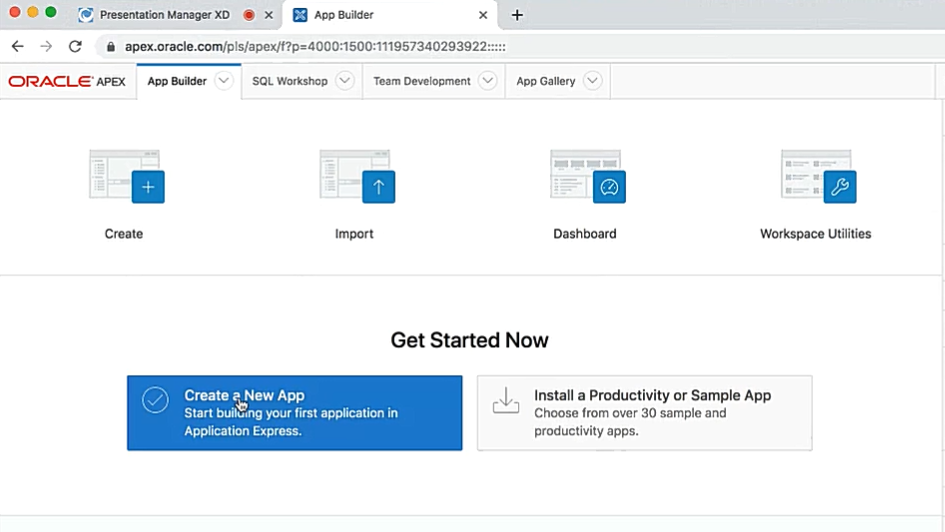
\includegraphics[scale=0.5]{figures/5}
    \caption{\textit{Create a New App}}
    \label{CreateApp}
\end{figure}
 \item Pilih menu From a File, menu ini memungkinkan kita memgupload data dari komputer kita dengan format csv, xml, dan xlsx.
 \begin{figure}[H]
    \centering
    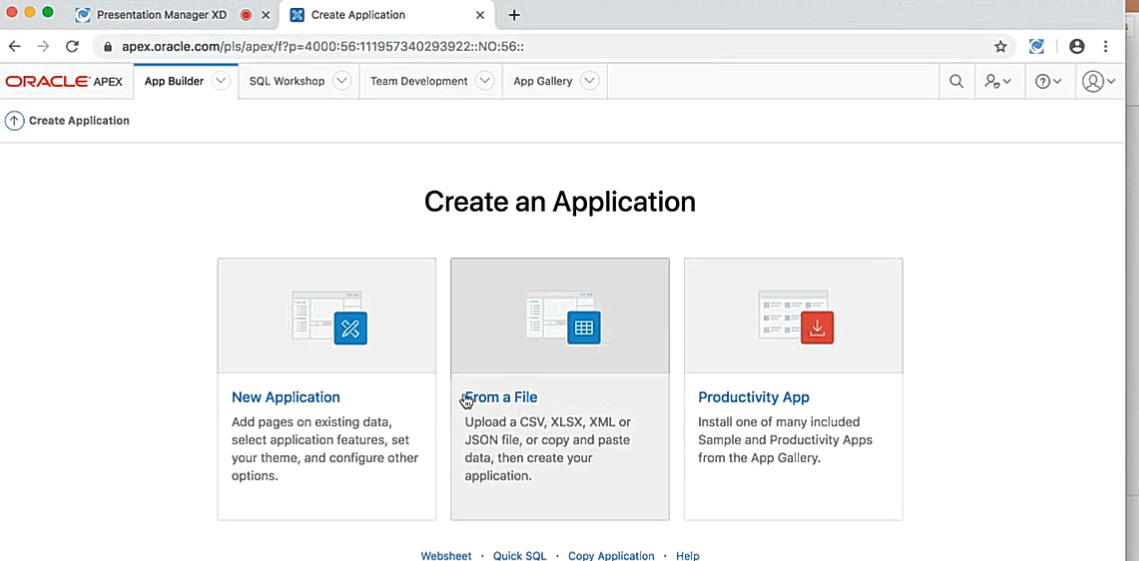
\includegraphics[scale=0.5]{figures/6}
    \caption{\textit{From A File}}
    \label{File}
\end{figure}
 \item Pilih menu Copy and Paste, menu ini memungkinkan kita menduplikasi file yang ada dikomputer kita dan menempelkan file tersebut pada apex.
 \begin{figure}[H]
    \centering
    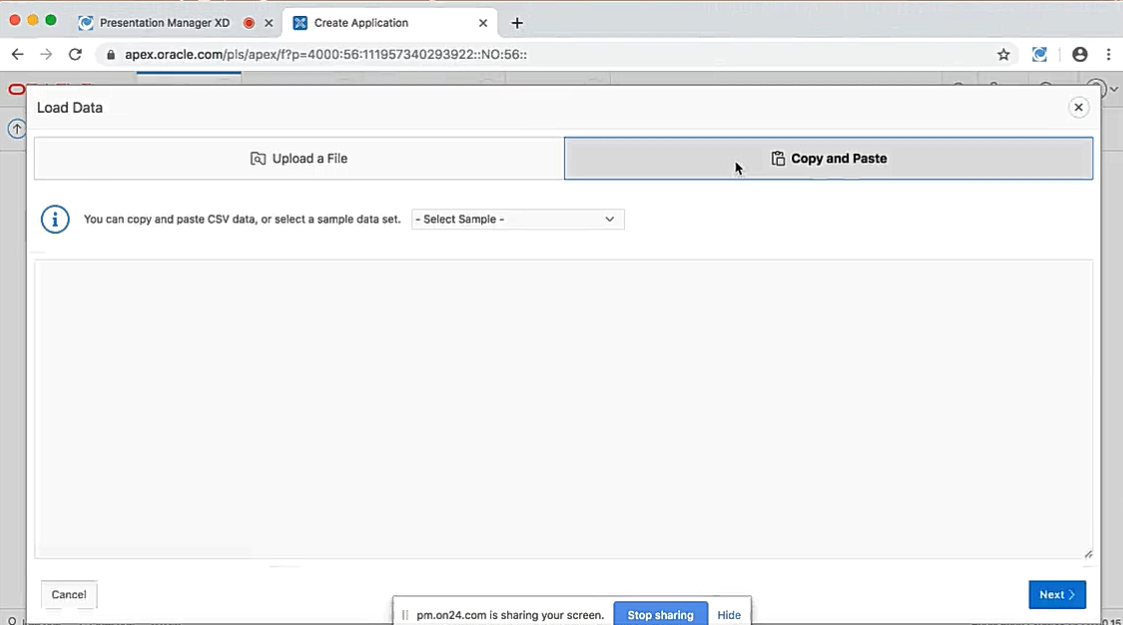
\includegraphics[scale=0.5]{figures/7}
    \caption{\textit{Copy And Paste}}
    \label{CopyPaste}
\end{figure}
 \item Pilih Data yang akan di Load.
 \begin{figure}[H]
    \centering
    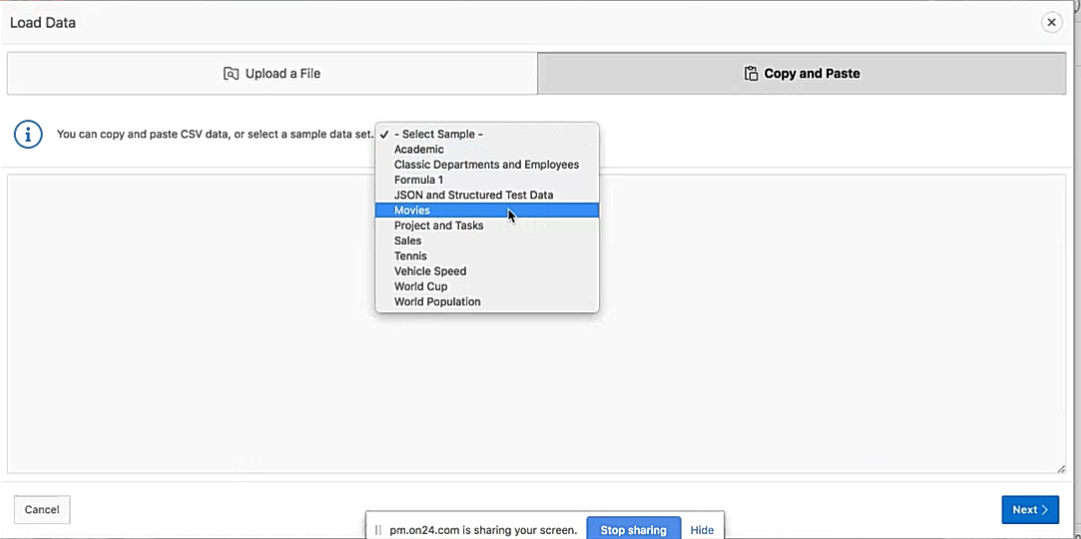
\includegraphics[scale=0.5]{figures/8}
    \caption{\textit{Load Data}}
    \label{LoadData}
\end{figure}
 \item Tampilan Data yang akan di Copy.
 \begin{figure}[H]
    \centering
    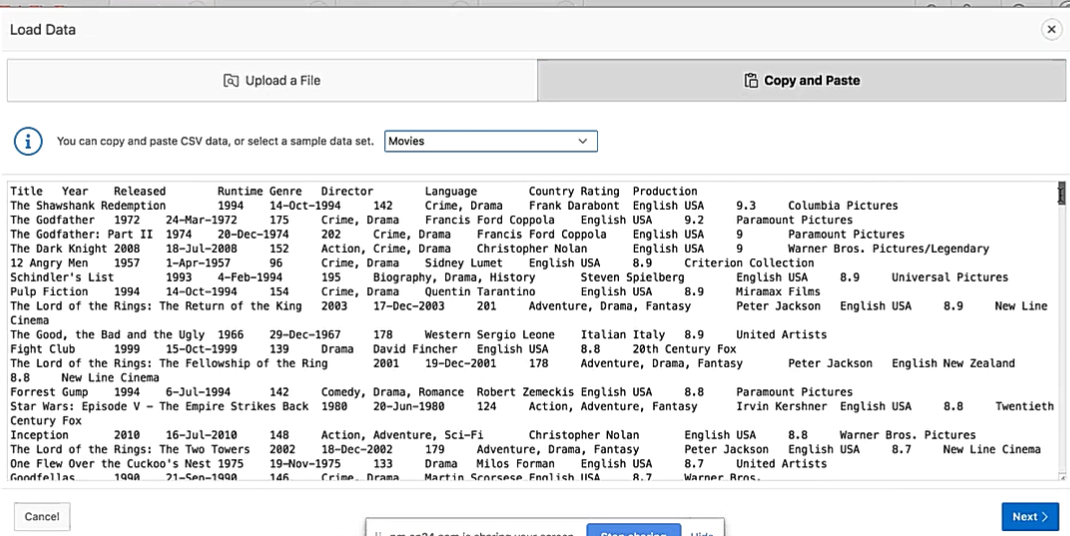
\includegraphics[scale=0.5]{figures/9}
    \caption{\textit{Copy Data}}
    \label{Data1}
\end{figure}
 \item Tampilan Data yang telah di Paste.
 \begin{figure}[H]
    \centering
    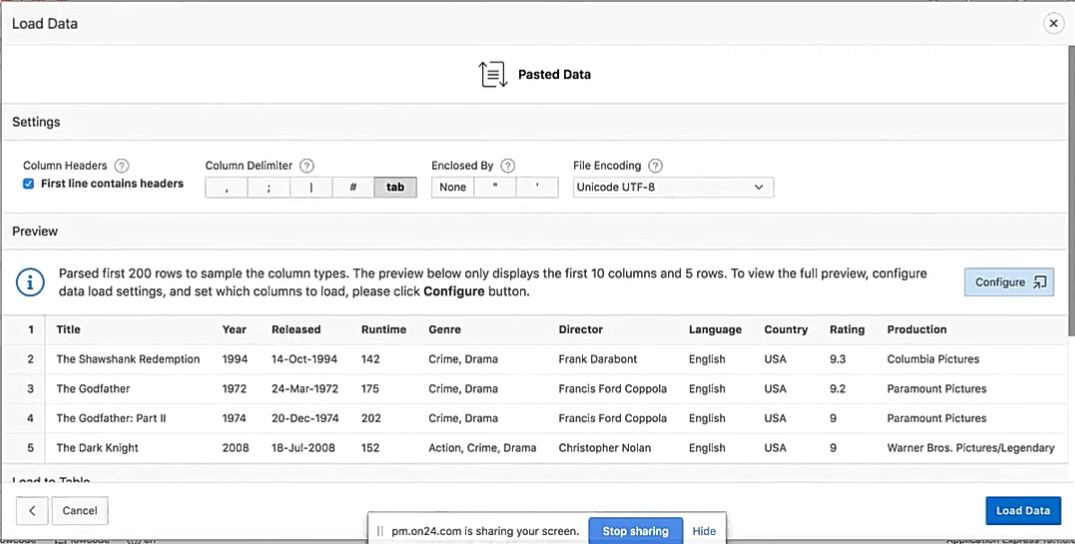
\includegraphics[scale=0.5]{figures/10}
    \caption{\textit{Paste Data}}
    \label{Data2}
\end{figure}
 \item Jika ingin melihat data pada database, dapat mengklik menu configure.
 \begin{figure}[H]
    \centering
    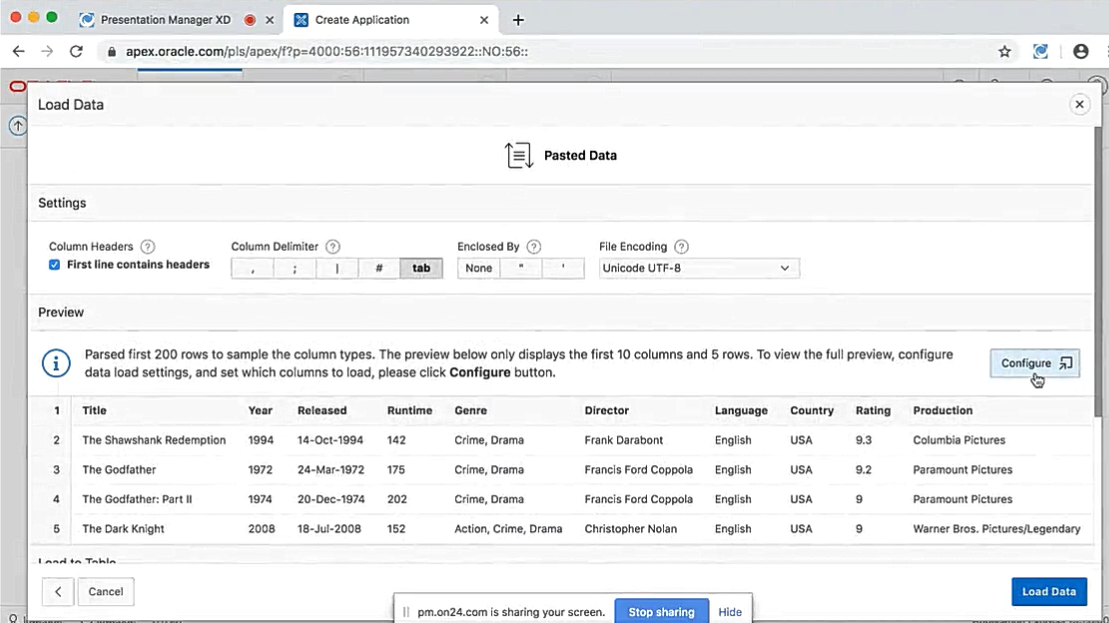
\includegraphics[scale=0.5]{figures/11}
    \caption{\textit{Configure}}
    \label{Configure}
\end{figure}
 \item Pilih menu columns to load, untuk melihat column pada database aplikasi.
 \begin{figure}[H]
    \centering
    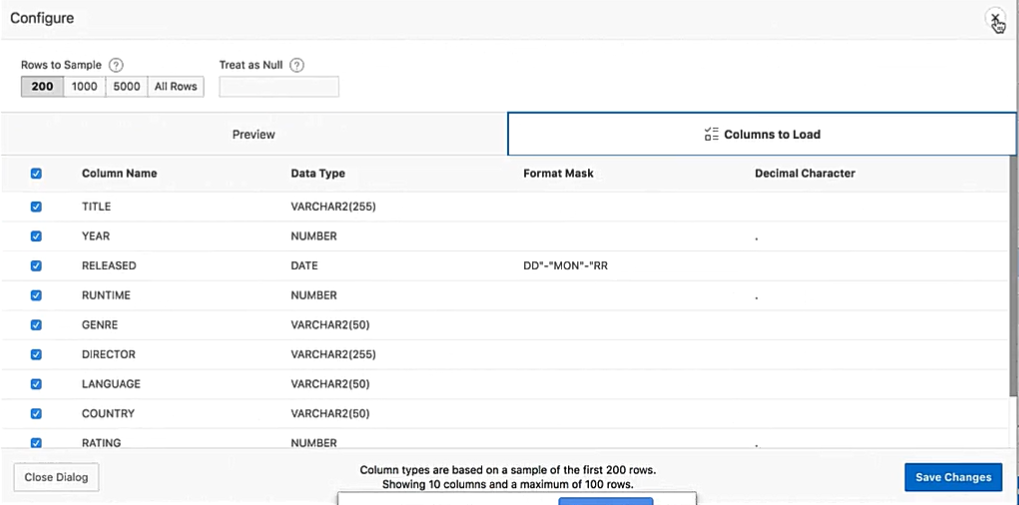
\includegraphics[scale=0.5]{figures/12}
    \caption{\textit{Columns To Load}}
    \label{Colums}
\end{figure}
 \item Scroll menu ke bawah, dan kemudian masukkan table name, error table name, kemudian klik next.
 \begin{figure}[H]
    \centering
    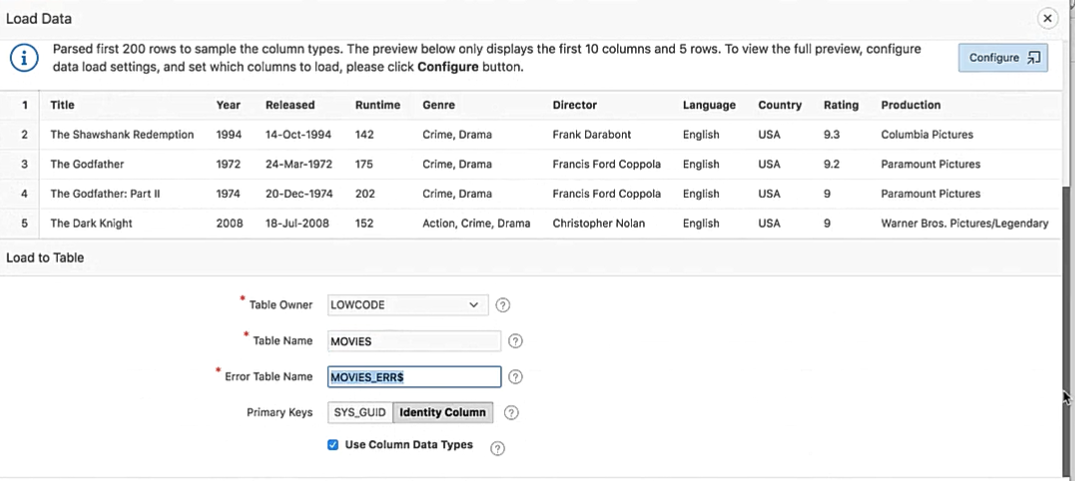
\includegraphics[scale=0.5]{figures/13}
    \caption{\textit{Data}}
    \label{Table}
\end{figure}
 \item Tampilan Data yang telah selesai di Load. Kemudian klik create application wizard.
 \begin{figure}[H]
    \centering
    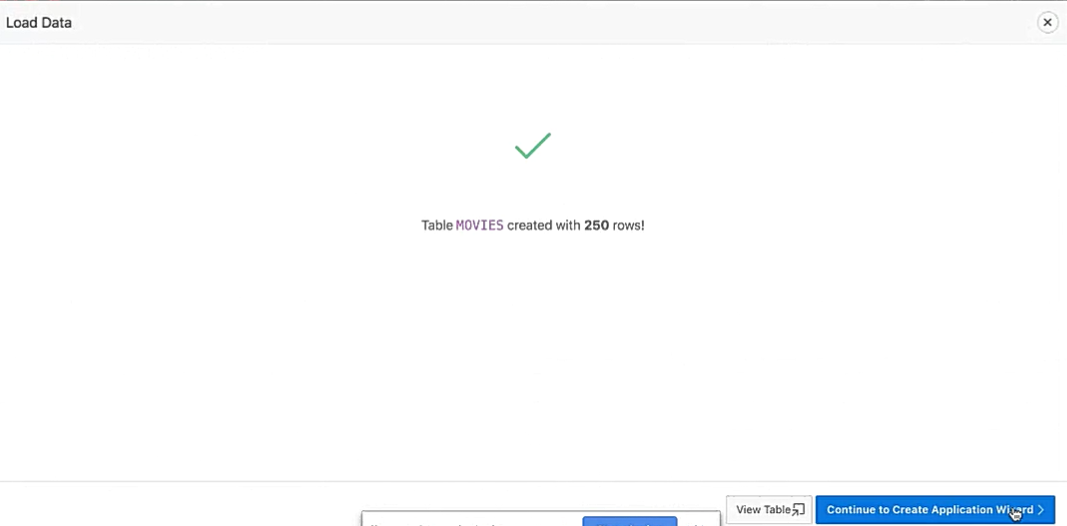
\includegraphics[scale=0.5]{figures/14}
    \caption{\textit{Load Data}}
    \label{Load Complete}
\end{figure}
 \item Pilih tampilan aplikasi yang diinginkan.
 \begin{figure}[H]
    \centering
    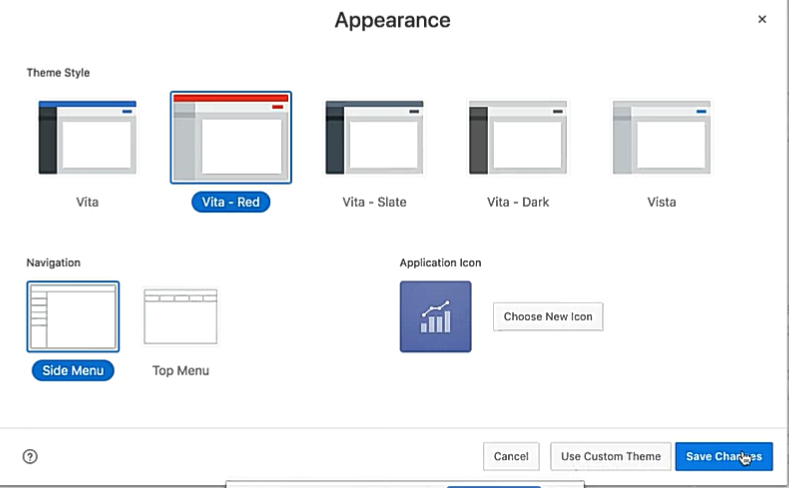
\includegraphics[scale=0.5]{figures/15}
    \caption{\textit{Appearance}}
    \label{Data}
\end{figure}
 \item Secara default akan terbentuk tiga halaman aplikasi, yaitu Home, Movies, dan Dashboard.
 \begin{figure}[H]
    \centering
    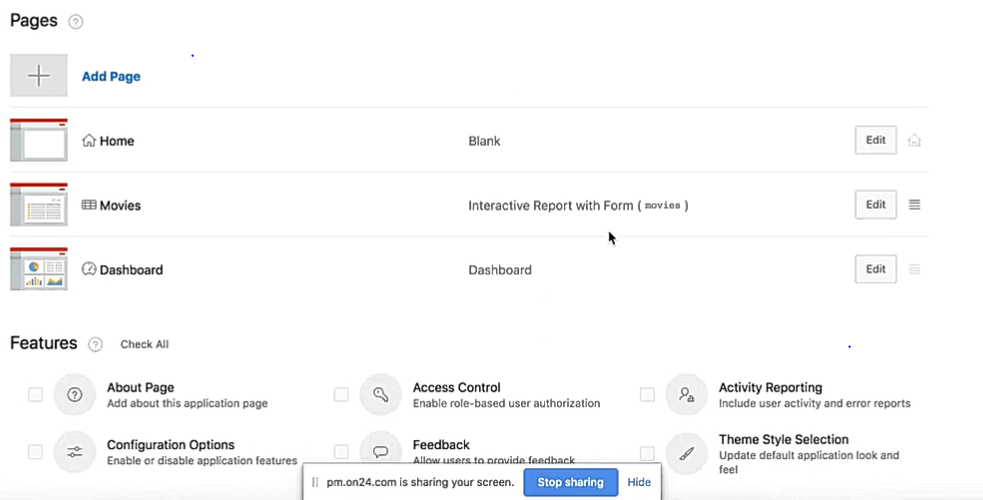
\includegraphics[scale=0.5]{figures/16}
    \caption{\textit{Pages}}
    \label{Page}
\end{figure}
 \item Scroll ke bawah, centang menu check all, lalu klik menu Create Application.
 \begin{figure}[H]
    \centering
    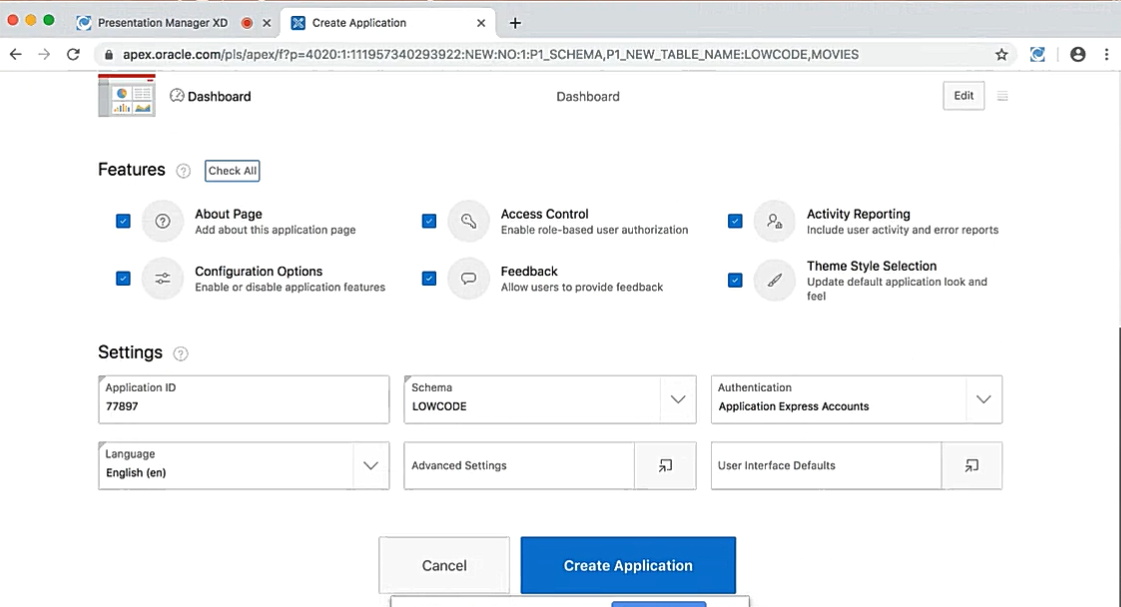
\includegraphics[scale=0.5]{figures/17}
    \caption{\textit{Data}}
    \label{CheckAll}
\end{figure}
\item Tunggu hingga proses pembuatan aplikasi selesai.
 \begin{figure}[H]
    \centering
    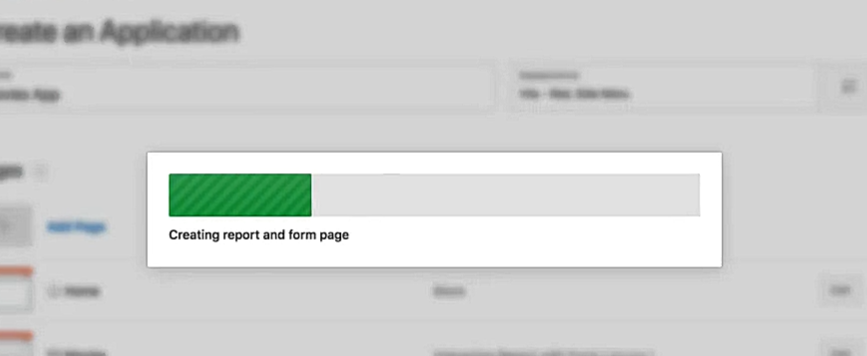
\includegraphics[scale=0.5]{figures/18}
    \caption{\textit{App Done}}
    \label{AppDone}
\end{figure}
\item Jika telah selesai, maka pilih menu Run Application.
 \begin{figure}[H]
    \centering
    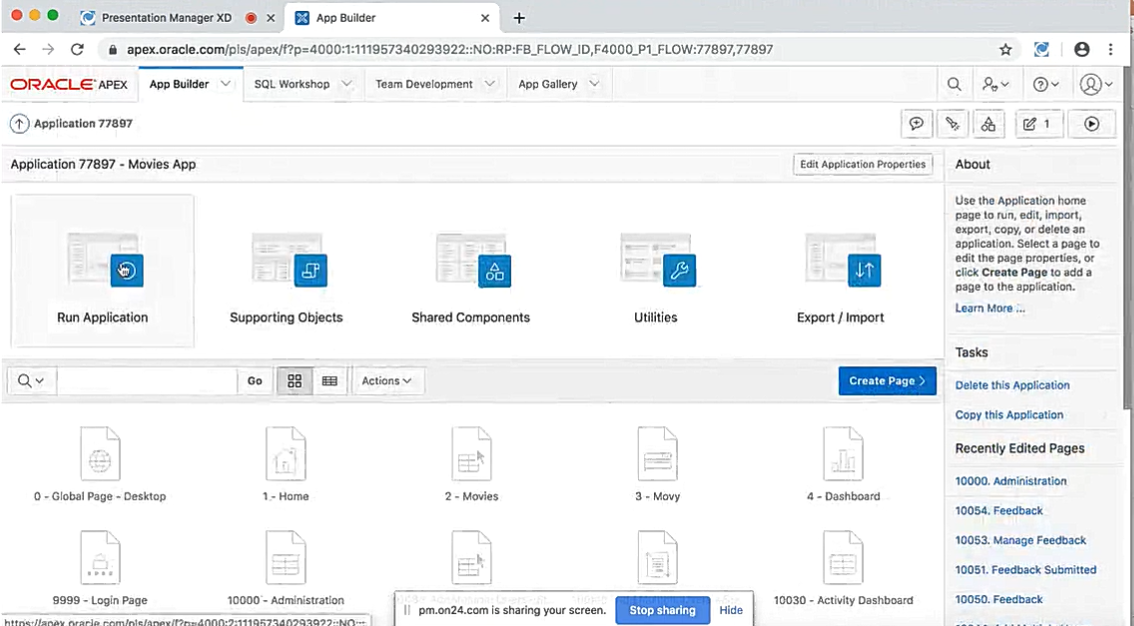
\includegraphics[scale=0.5]{figures/19}
    \caption{\textit{Run Application}}
    \label{RunApp}
\end{figure}
\item Masukkan Username dan Password App.
 \begin{figure}[H]
    \centering
    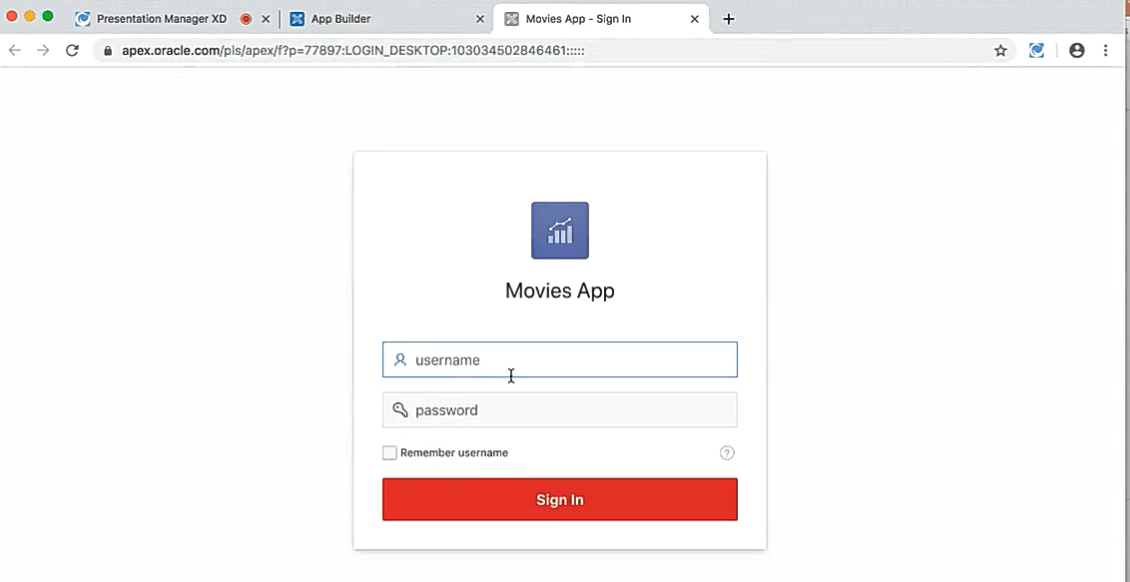
\includegraphics[scale=0.5]{figures/20}
    \caption{\textit{Login App}}
    \label{LoginApp}
\end{figure}
\item Tampilan Home aplikasi Movies App.
 \begin{figure}[H]
    \centering
    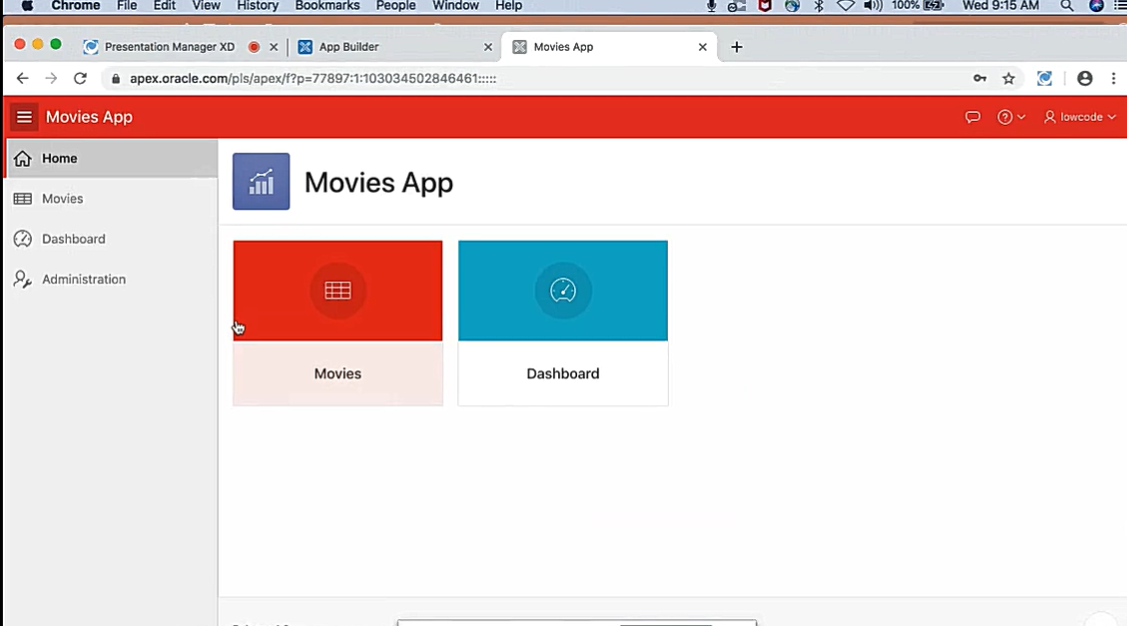
\includegraphics[scale=0.5]{figures/21}
    \caption{\textit{Menu Home}}
    \label{Menu1}
\end{figure}
\item Tampilan data yang telah diLoad akan muncul pada menu Movies pada aplikasi Movies App.
 \begin{figure}[H]
    \centering
    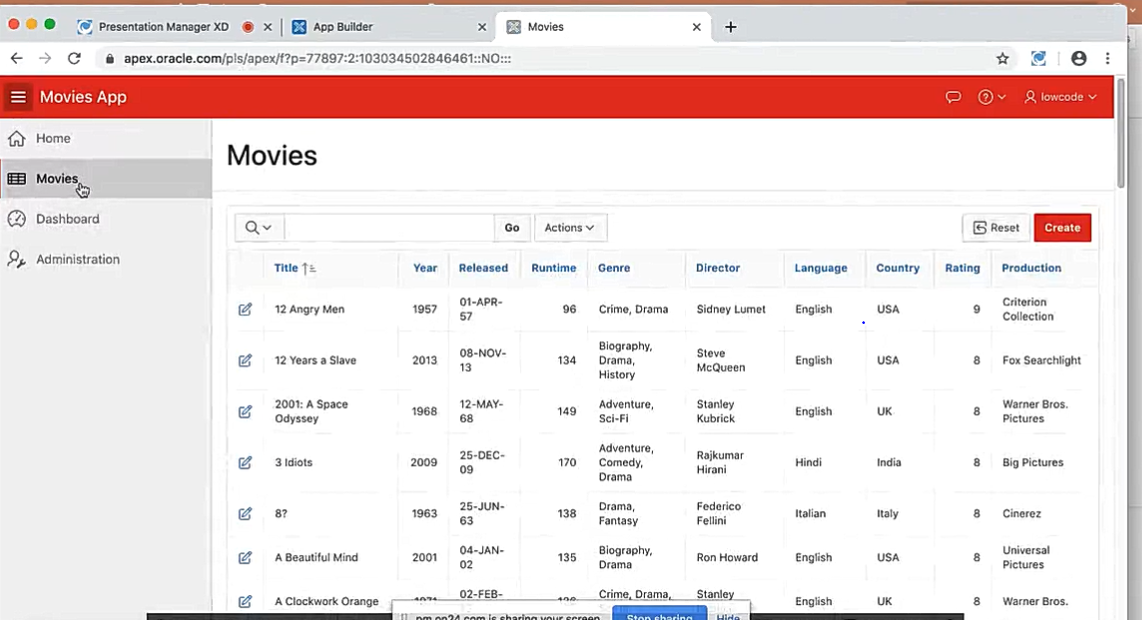
\includegraphics[scale=0.5]{figures/22}
    \caption{\textit{Menu Movies}}
    \label{Menu2}
\end{figure}
\item Aplikasi telah selesai dibuat, dan dapat dijalankan dengan baik.
\end{enumerate}

\subsection{Kegunaan APEX}
\begin{enumerate}
 \item Pengganti speadsheet. Sebagai pengganti spreadsheet, apex oracle memiliki fitur drag and drop untuk data yang bertipe csv, xls, xml, or json file. Membuat tabel database outonomous. Memungkinkan kita mengupload data kedalam tabel baru. Membuat aplikasi berdasarkan tabel baru.
 \item Pembuatan Oracle form yang modern. fitur yang dimiliki oracle yaitu form yang natural, tidak terlalu rumit. Support SQL maupun PL/SQL. Dapat menggunakan kembali paket database, prosedur dan fungsi. Dapat Dengan mudah mengembangkan form dari satu developer ke developer lain.
 \item Pengembangan aplikasi secara cepat. Dengan apex kita bisa membuat aplikasi dalam hitungan hari atau minggu, tidak akan membutuhkan waktu bertahun-tahun. Sebagai penyihir hebat untuk membuat aplikasi berfitur lengkap. Merubah persyaratan dengan sangat mudah. Beralih dengan cepat ke aplikasi siap produksi. Kemampuan Low Code yang membuat pekerja non-IT bisa membantu dalam menggunakan apex dan membangun sebuah aplikasi.
 \item Membangun aplikasi skala perusahaan besar. Cepat dalam membangun aplikasi yang besar. Melaporkan dan Memperbaiki data perusahaan. Memungkinkan untuk memisahkan data silo. Membangun data laporan organisasi.
 \item Memperluas sistem perusahaan. Memperpanjang ERP dan sistem perangkat lunak lainnya. Menyediakan dashboard khusus organisasi. Meningkatkan alur kerja. Mengisi kekosongan.
\end{enumerate}

\subsection{Membuat Productivity App}
Selain dengan membuat aplikasi dengan data spreadsheet, kita juga bisa membuat aplikasi dengan menggunakan Productivity App yang mana didalamnya telah terdapat berbagai macam aplikasi yang bisa kita gunakan sebagai aplikasi kita.\\
Berikut langkah-langkah membuat prodictivity app.
\begin{enumerate}
 \item Pertama, klik App Build. kemudian pilih Productivity App
 \begin{figure}[H]
    \centering
    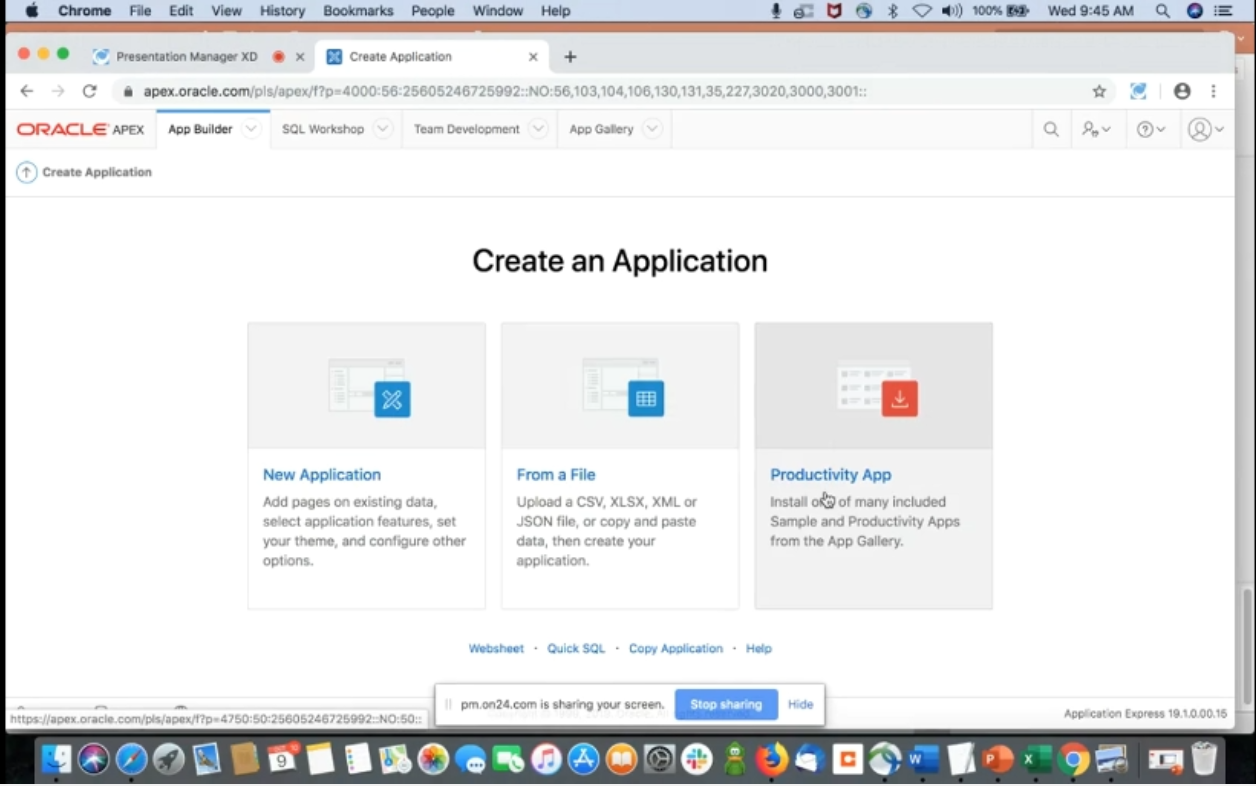
\includegraphics[scale=0.5]{figures/a}
    \caption{\textit{App Build}}
    \label{foto1}
\end{figure}
 \item Kemudian, pilih aplikasi yang akan di buat
 \begin{figure}[H]
    \centering
    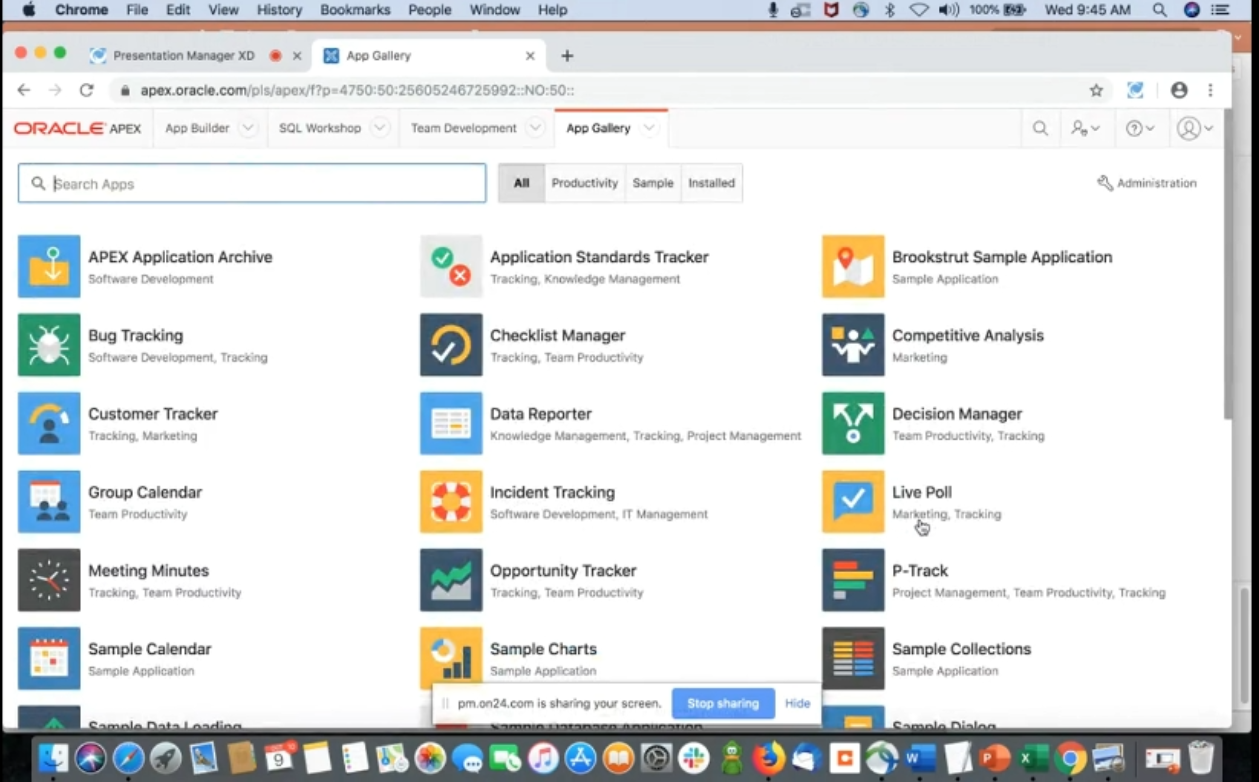
\includegraphics[scale=0.5]{figures/b}
    \caption{\textit{Choose App}}
    \label{foto2}
\end{figure}
 \item Sebagai contoh pilih Sample Charts
 \begin{figure}[H]
    \centering
    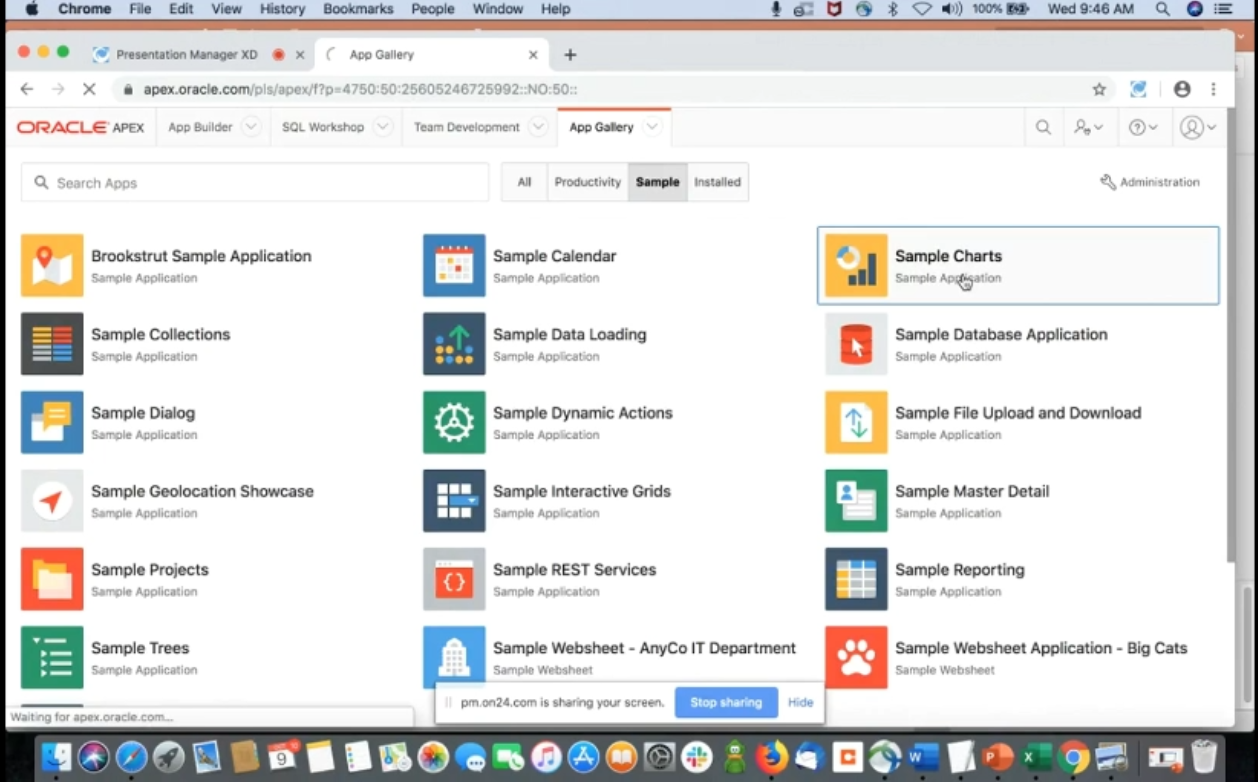
\includegraphics[scale=0.5]{figures/c}
    \caption{\textit{Sample Charts}}
    \label{foto3}
\end{figure}
 \item Klik install app
 \begin{figure}[H]
    \centering
    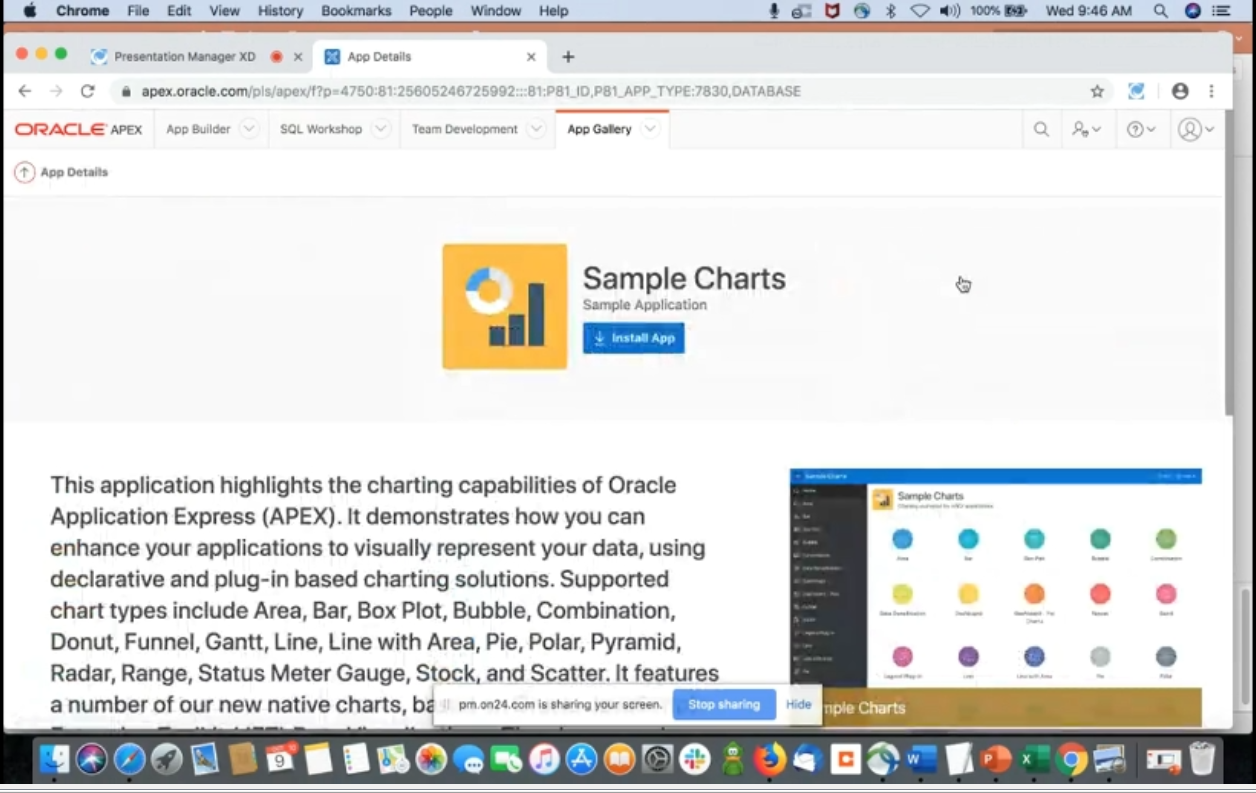
\includegraphics[scale=0.5]{figures/d}
    \caption{\textit{Install App}}
    \label{foto4}
\end{figure}
 \item Kemudian pilih next untuk melanjutkan instalasi.
 \begin{figure}[H]
    \centering
    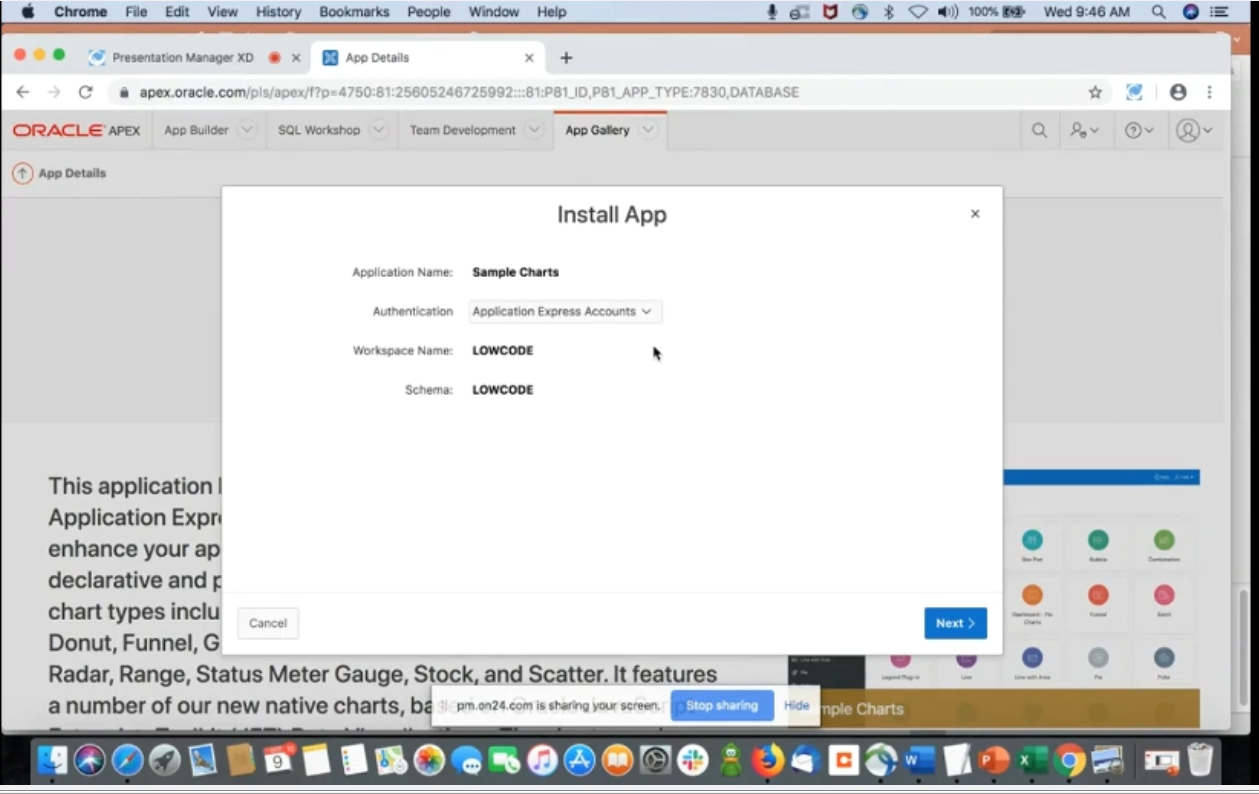
\includegraphics[scale=0.5]{figures/e}
    \caption{\textit{Next}}
    \label{foto5}
\end{figure}
 \item Klik install app.
 \begin{figure}[H]
    \centering
    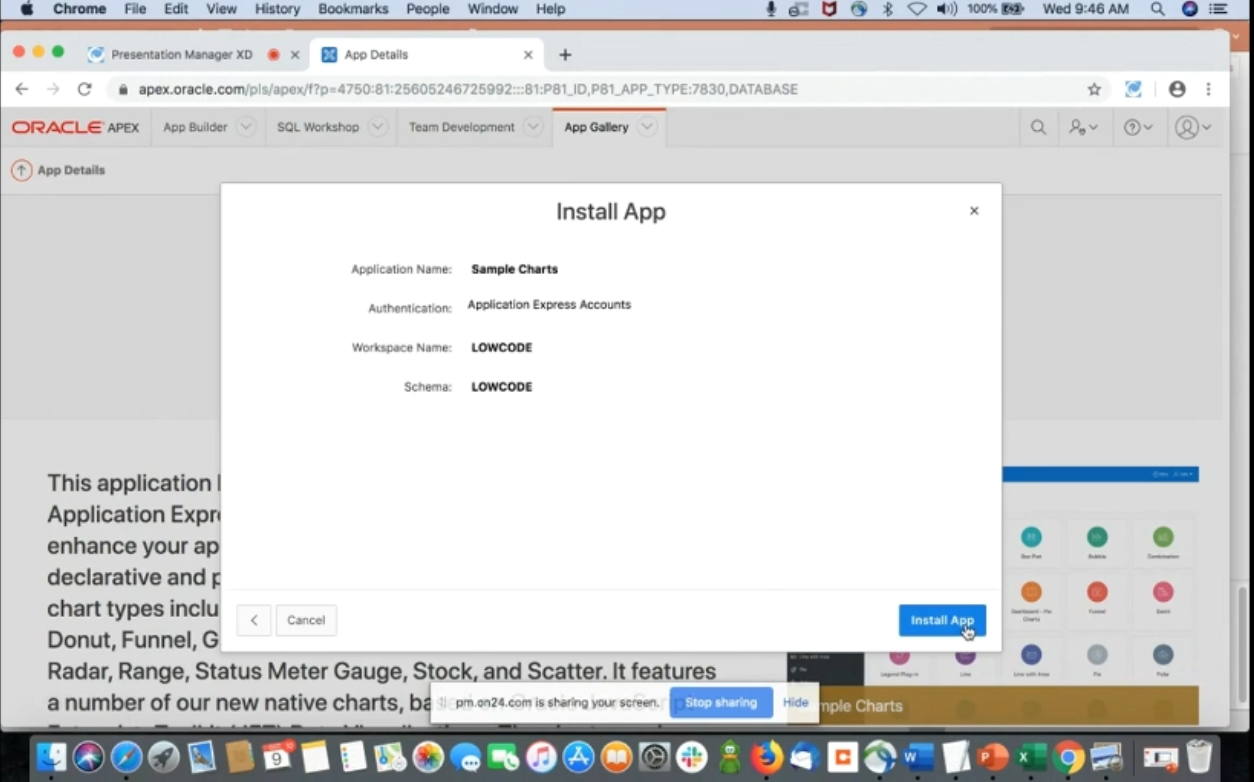
\includegraphics[scale=0.5]{figures/f}
    \caption{\textit{Install}}
    \label{foto6}
\end{figure}
 \item Tunggu hingga proses instalasi selesai.
 \begin{figure}[H]
    \centering
    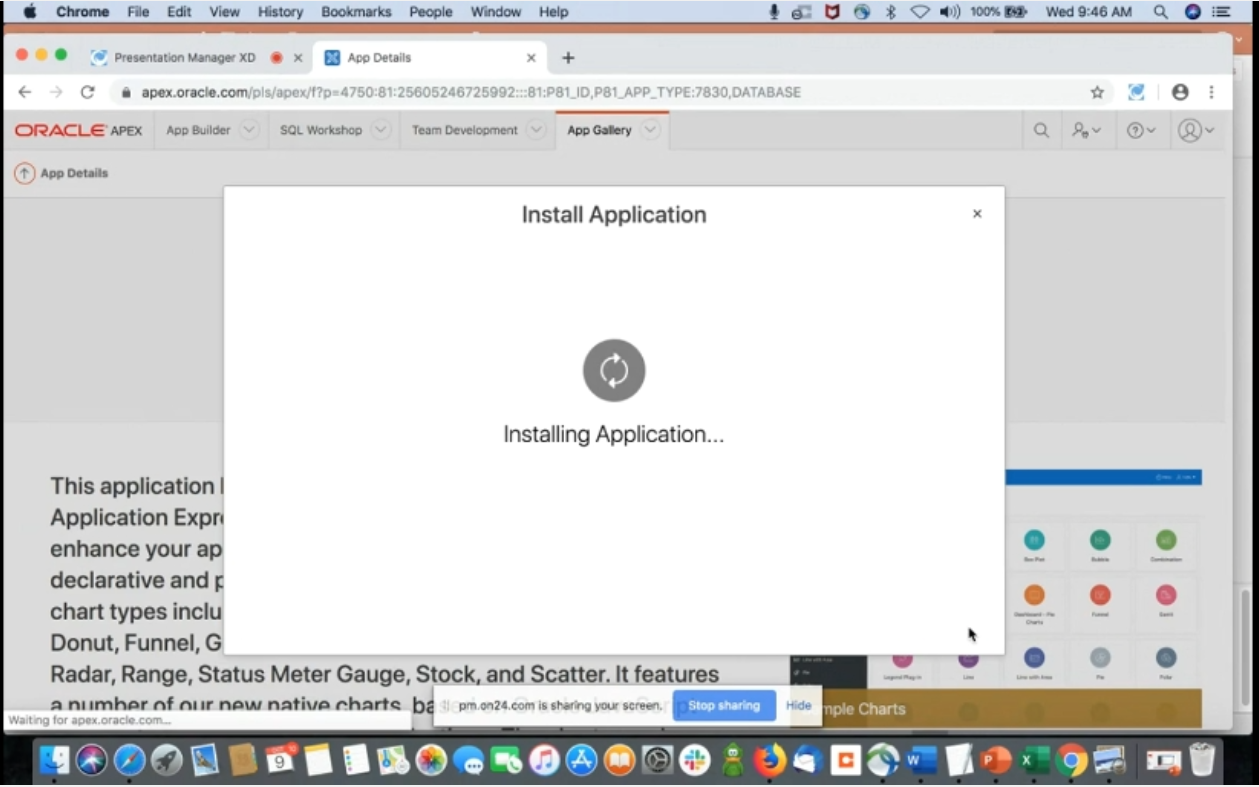
\includegraphics[scale=0.5]{figures/g}
    \caption{\textit{Wait}}
    \label{foto7}
\end{figure}
 \item Jika sudah selesai, maka jalankan aplikasi.
 \begin{figure}[H]
    \centering
    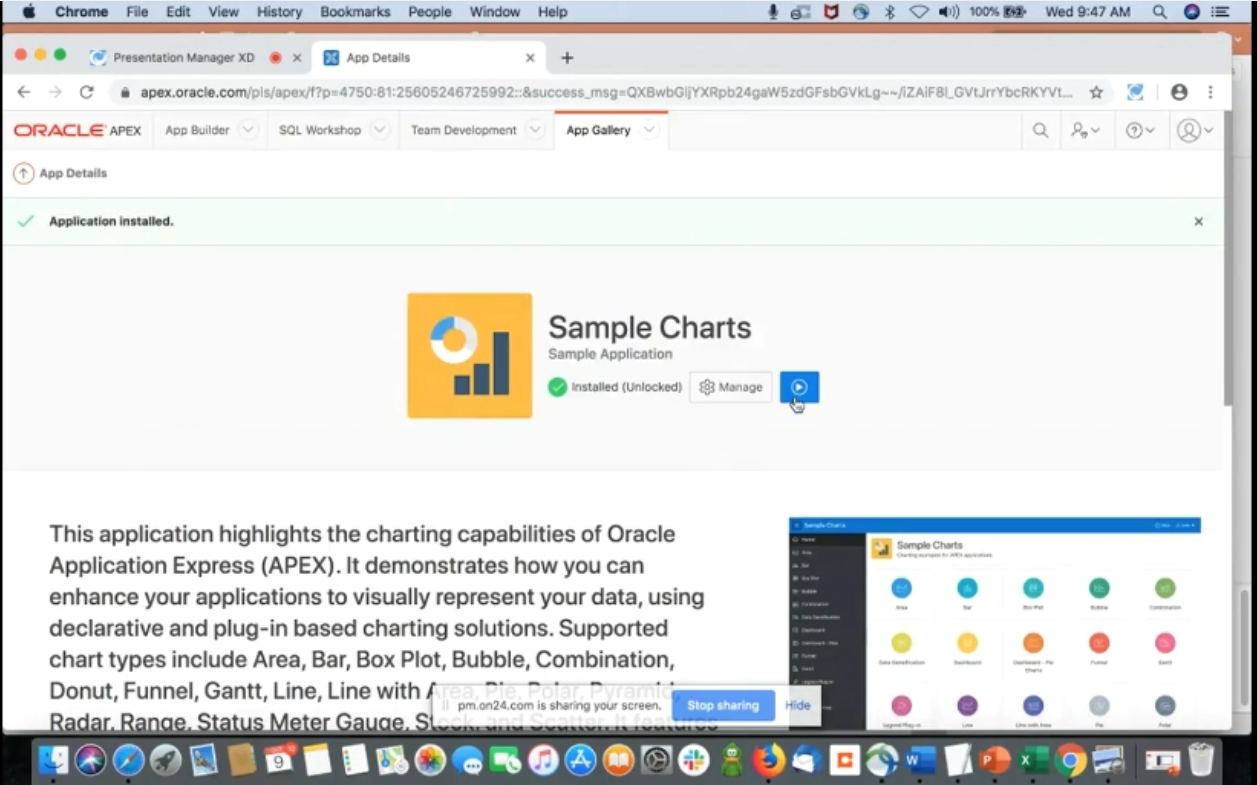
\includegraphics[scale=0.5]{figures/h}
    \caption{\textit{Run}}
    \label{foto8}
\end{figure}
 \item Login menggunakan account oracle.
 \begin{figure}[H]
    \centering
    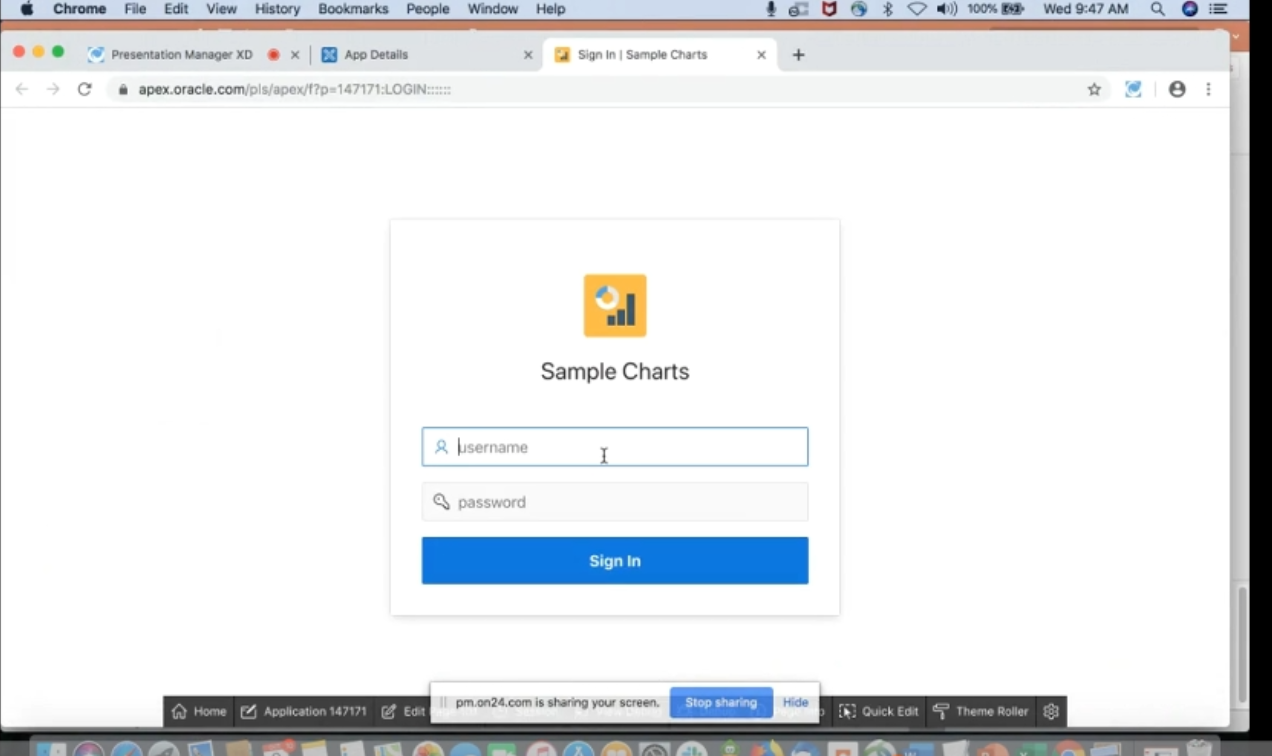
\includegraphics[scale=0.5]{figures/i}
    \caption{\textit{Login}}
    \label{foto9}
\end{figure}
\item Maka kita telah berhasil membuat aplikasi sample charts.
 \begin{figure}[H]
    \centering
    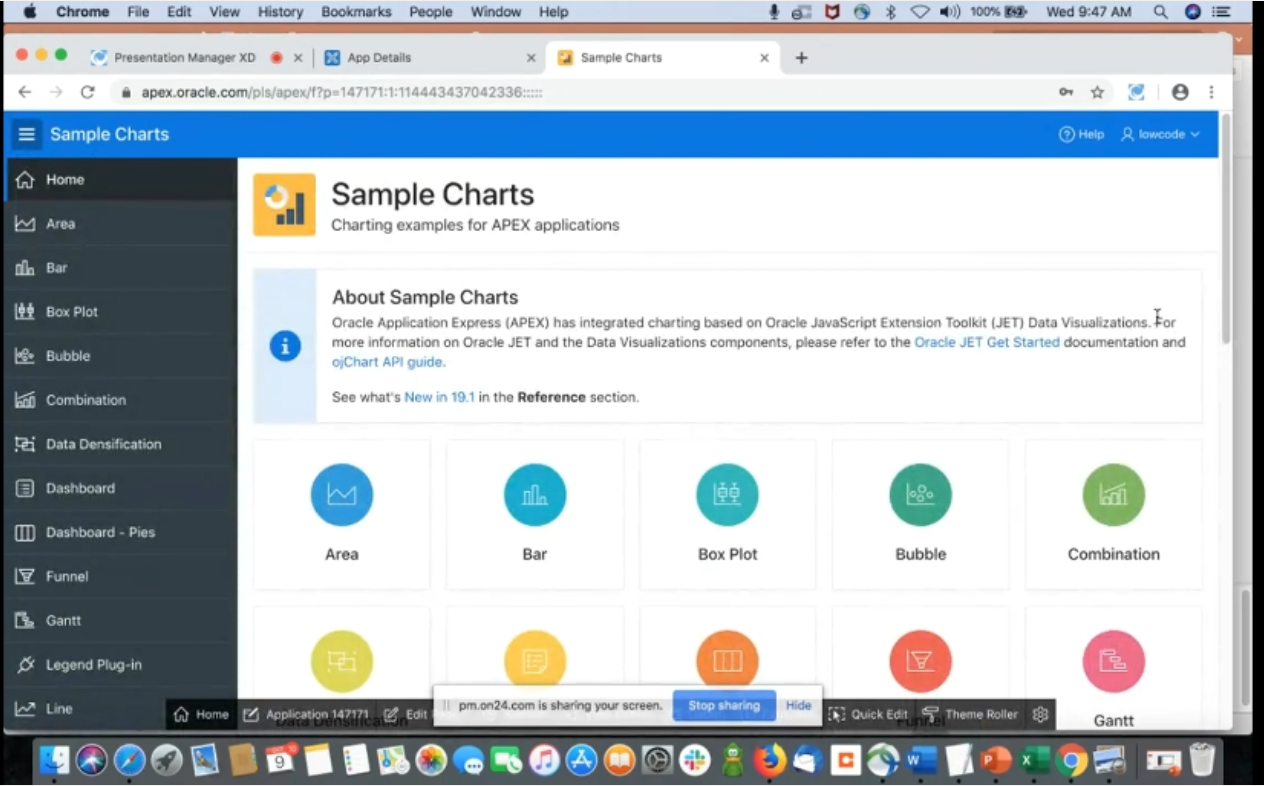
\includegraphics[scale=0.5]{figures/j}
    \caption{\textit{Succes}}
    \label{foto10}
\end{figure}
 \item Selanjutnya, akan diperkenalkan masing-masing menu yang ada di oracle apex. Menu yang pertama yaitu menu Object Browser. Pada menu ini kita bisa melihat tabel-tabel yang telah kita buat.
 \begin{figure}[H]
    \centering
    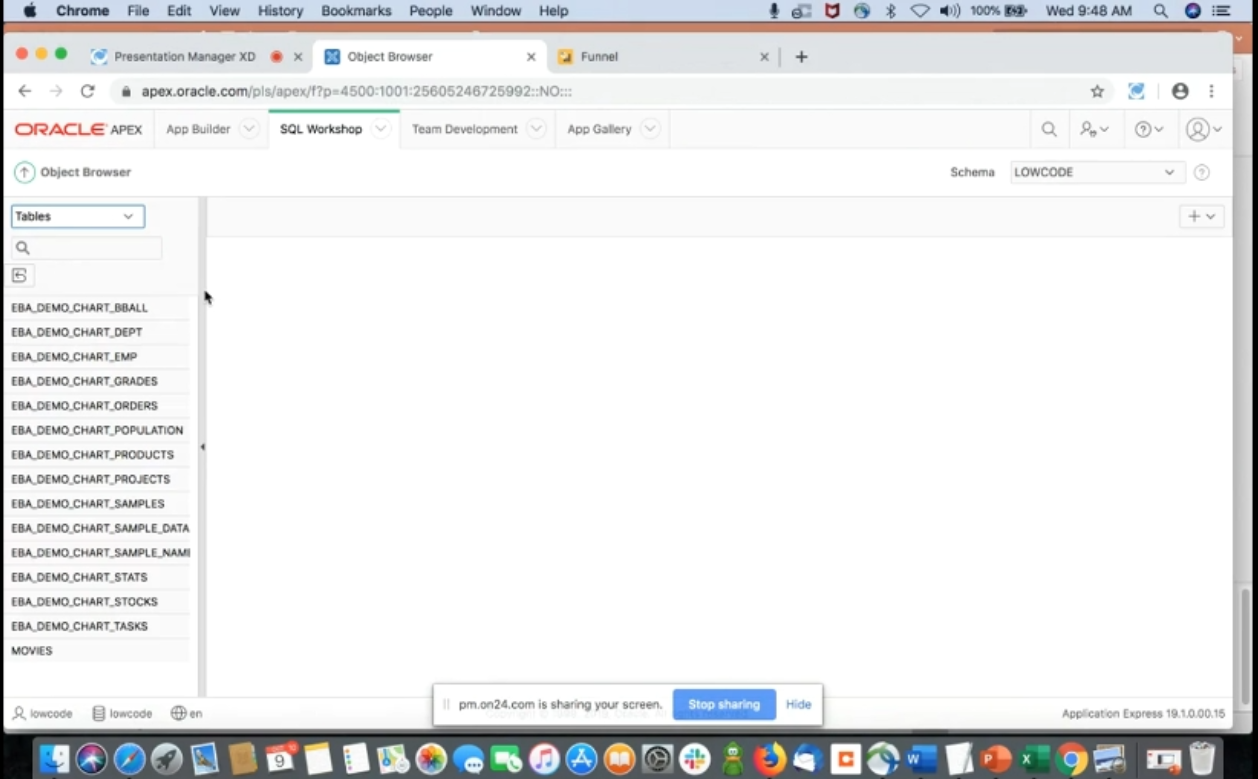
\includegraphics[scale=0.5]{figures/k}
    \caption{\textit{Menu Object Browser}}
    \label{foto11}
\end{figure}
 \item Apabila kita klik salah satu tabel, maka akan muncul data column yang ada pada tabel tersebut.
 \begin{figure}[H]
    \centering
    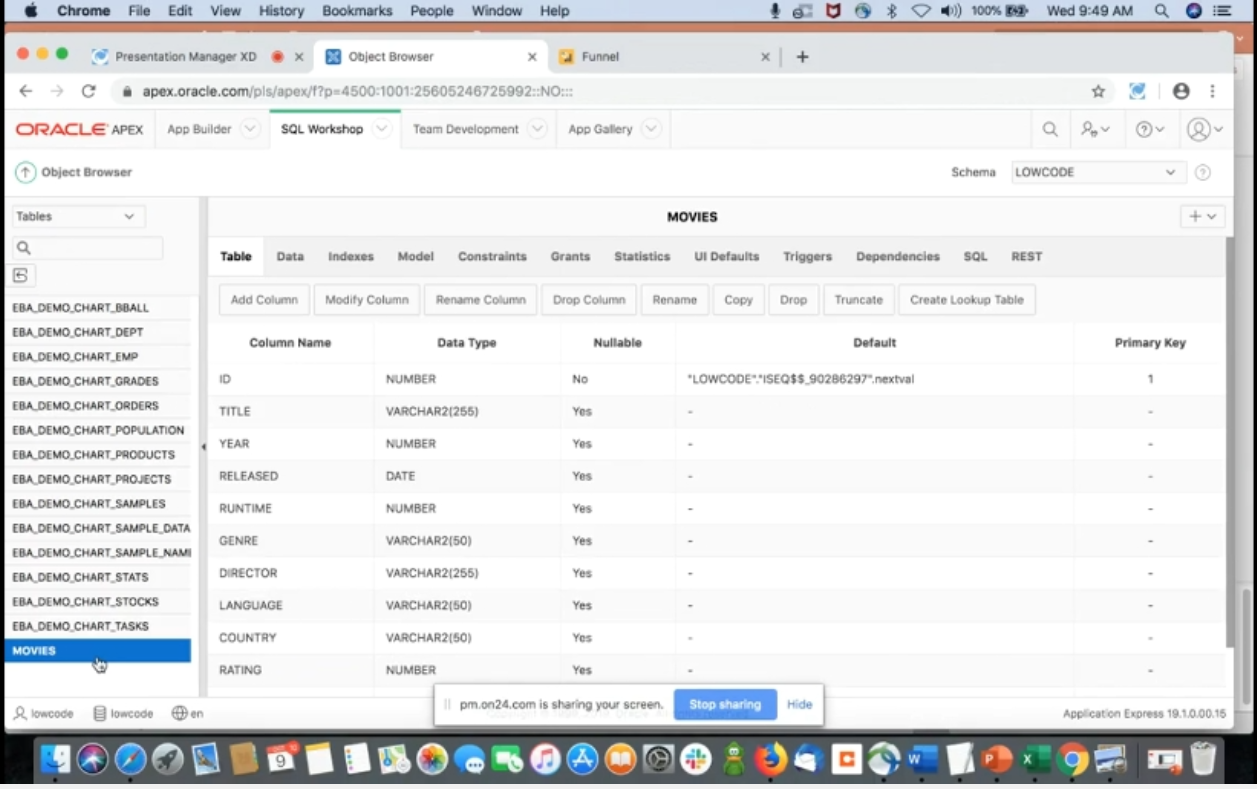
\includegraphics[scale=0.5]{figures/l}
    \caption{\textit{Data Column}}
    \label{foto12}
\end{figure}
 \item Menu yang kedua yaitu SQL Commands, menu ini berfungsi sebagai tempat pengetikan perintah SQL.
 \begin{figure}[H]
    \centering
    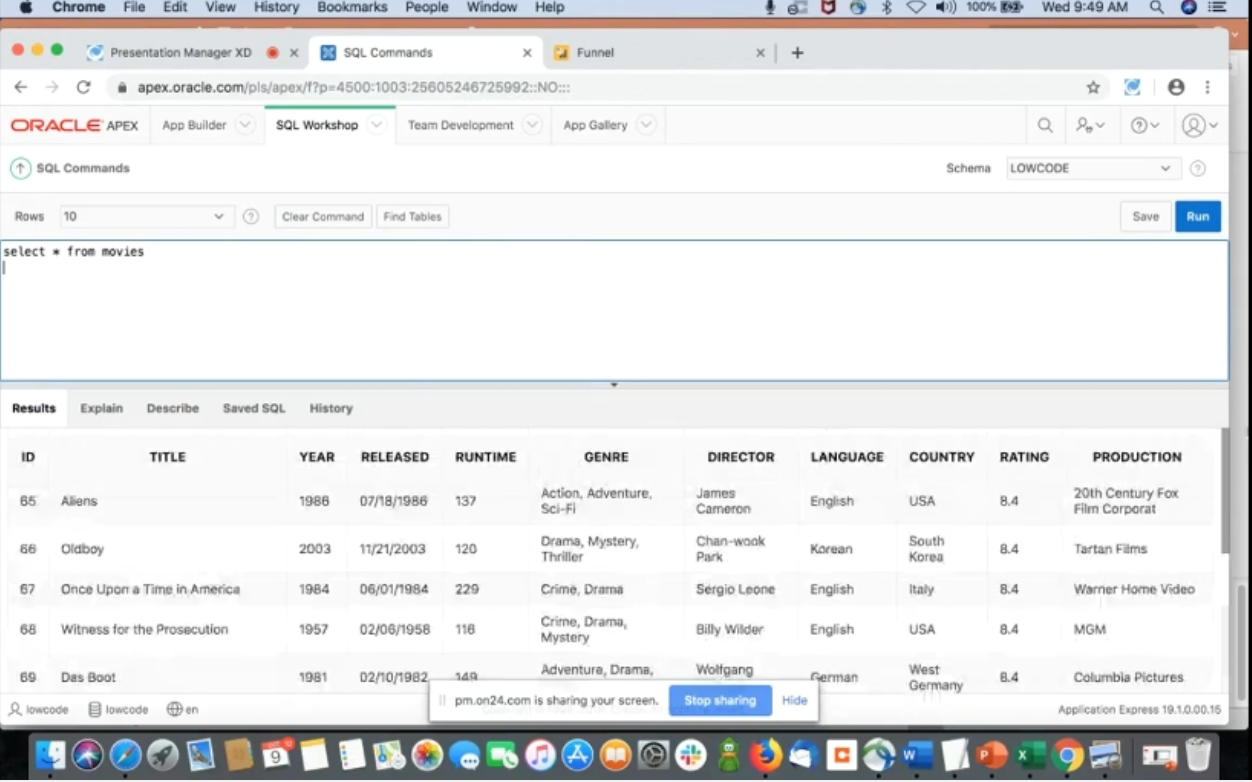
\includegraphics[scale=0.5]{figures/m}
    \caption{\textit{SQL Command}}
    \label{foto13}
\end{figure}
\item Menu selanjutnya yaitu Utilities. Pada menu ini kita bisa melihat semua yang telah kita kerjakan/ proyek yang sedang kita kerjakan, kita juga bisa menjalankan program melalui utilities.
 \begin{figure}[H]
    \centering
    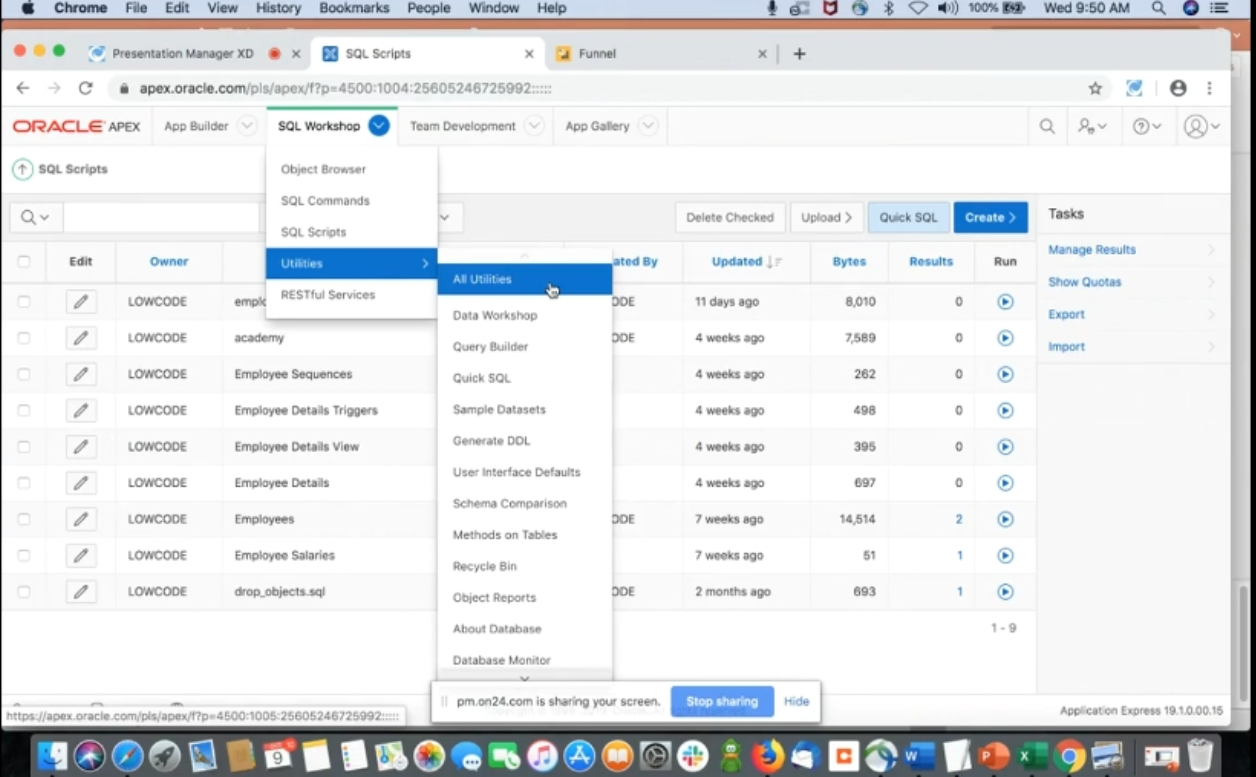
\includegraphics[scale=0.5]{figures/o}
    \caption{\textit{Utilities}}
    \label{foto15}
\end{figure}
\item Menu selanjutnya yaitu Data load/unload berfungsi untuk memasukkan data ke apex atau membongkar data yang ada di apex.
 \begin{figure}[H]
    \centering
    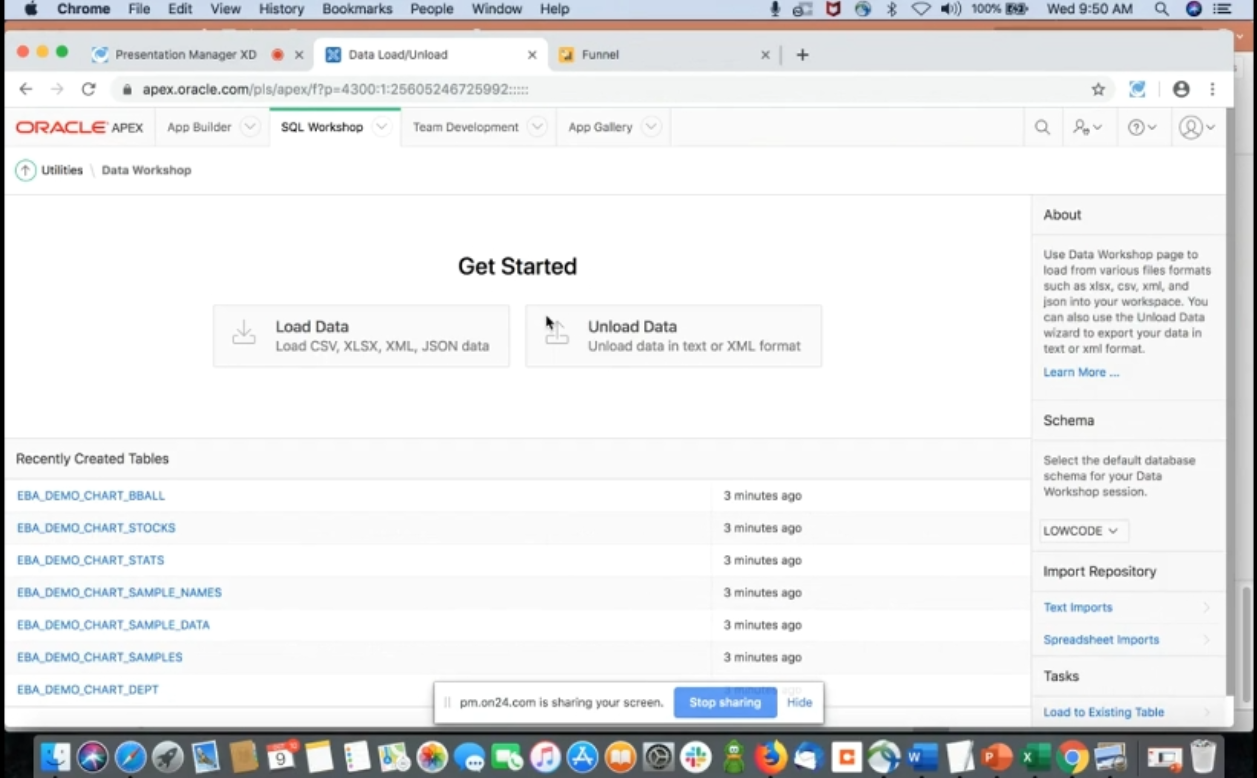
\includegraphics[scale=0.5]{figures/p}
    \caption{\textit{Data Load/Unload}}
    \label{foto16}
\end{figure}
\item Apabila kita mengklik load data maka akan muncul menu uplod file, kita bisa memasukkan data kita dengan format csv, xlsx, txt, xml, dan json.
 \begin{figure}[H]
    \centering
    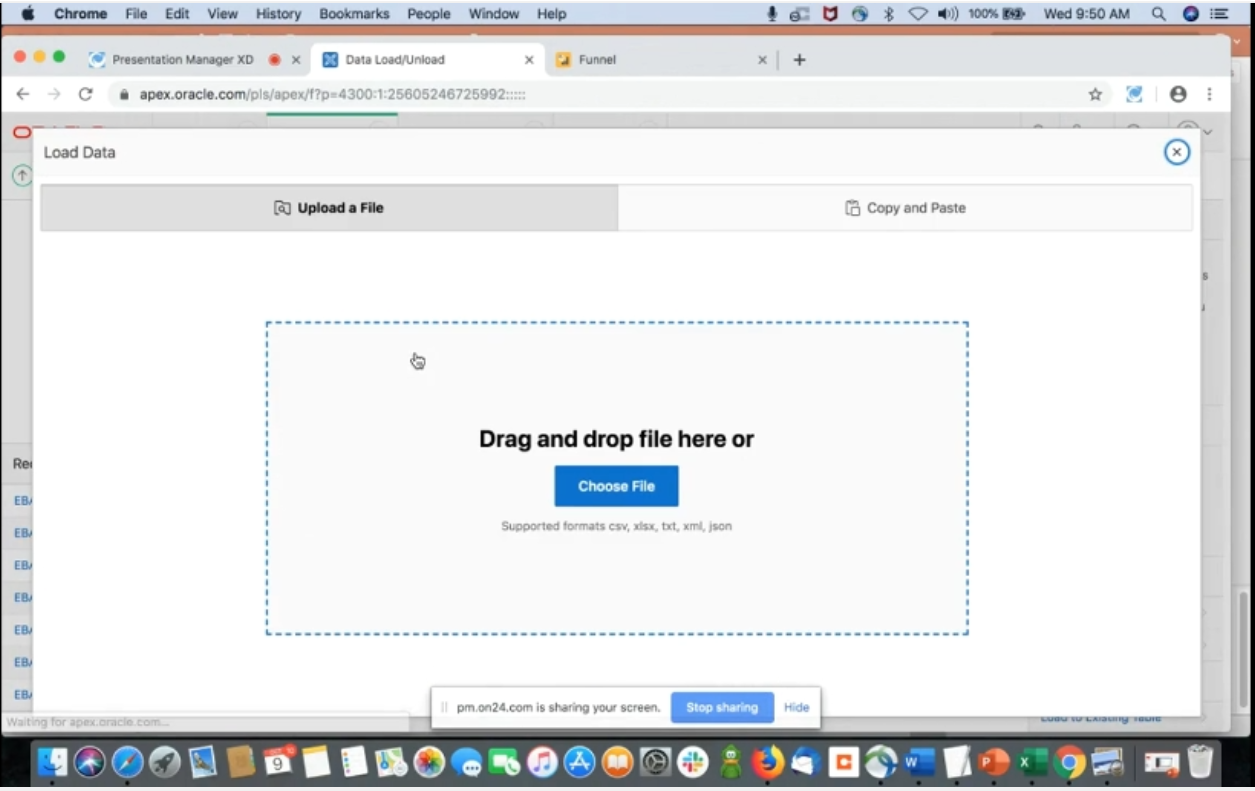
\includegraphics[scale=0.5]{figures/q}
    \caption{\textit{Load File}}
    \label{foto17}
\end{figure}
\item Menu Quick SQL berguna untuk membuat database dengan perintah kode yang minim dan cepat.
 \begin{figure}[H]
    \centering
    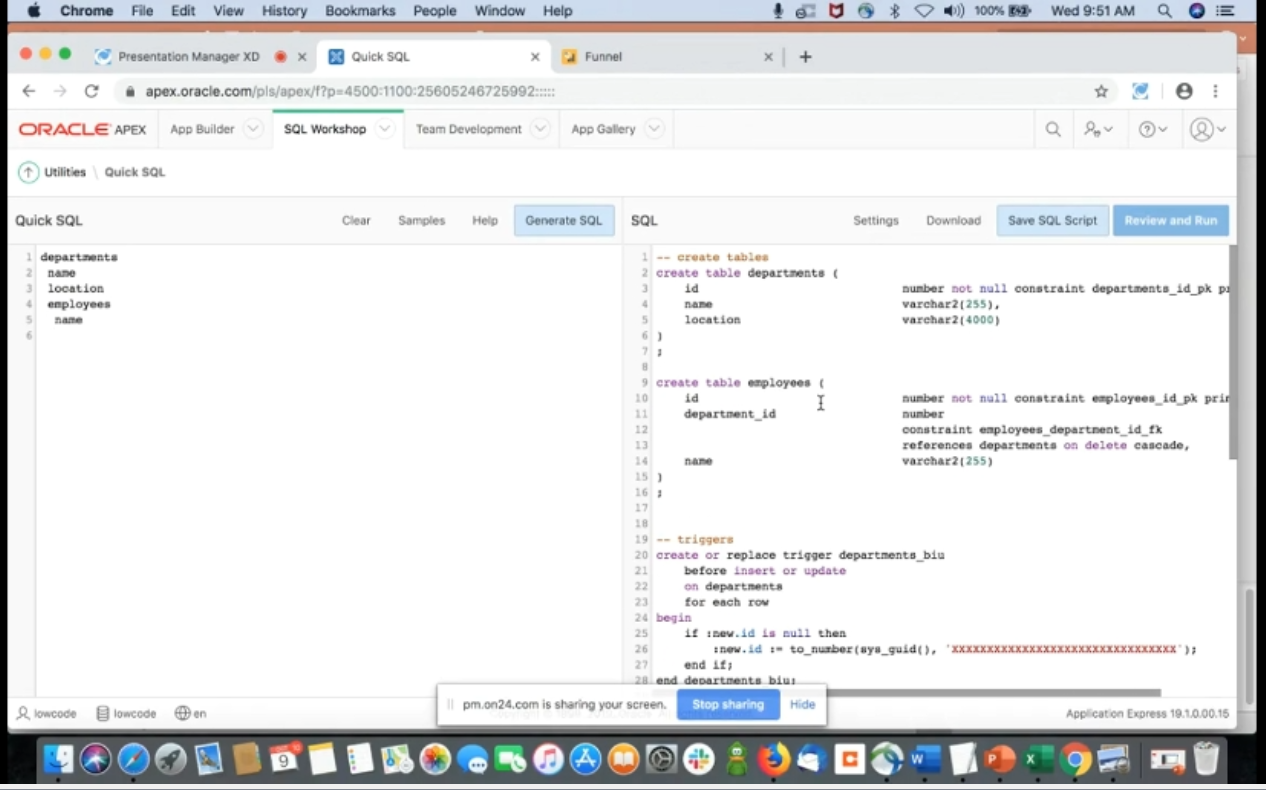
\includegraphics[scale=0.5]{figures/s}
    \caption{\textit{Quick SQL}}
    \label{foto19}
\end{figure}
\item Pada Quick SQL kita juga bisa mengambil sample data sebagai acuan dalam membuat database.
 \begin{figure}[H]
    \centering
    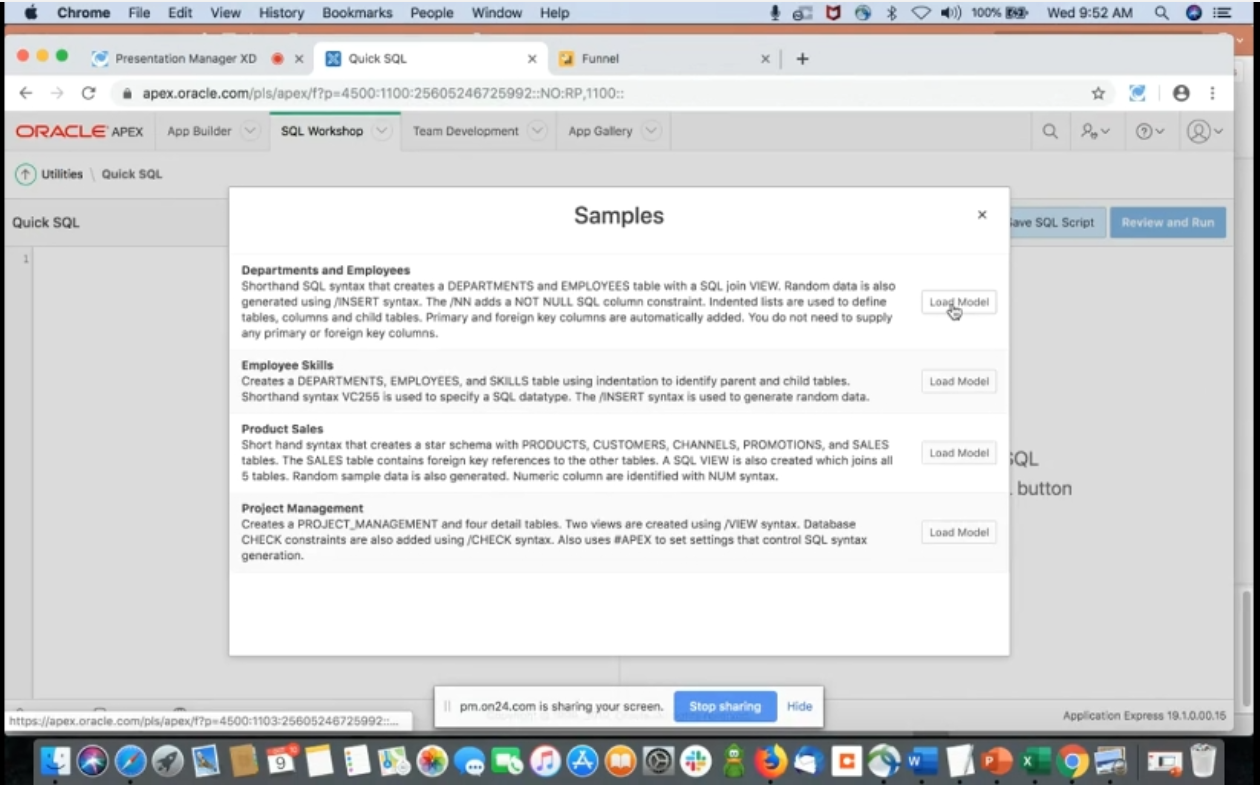
\includegraphics[scale=0.5]{figures/t}
    \caption{\textit{Sample Data}}
    \label{foto20}
\end{figure}
\item Tampilan Sample database yang bisa kita edit pada Quick SQL
 \begin{figure}[H]
    \centering
    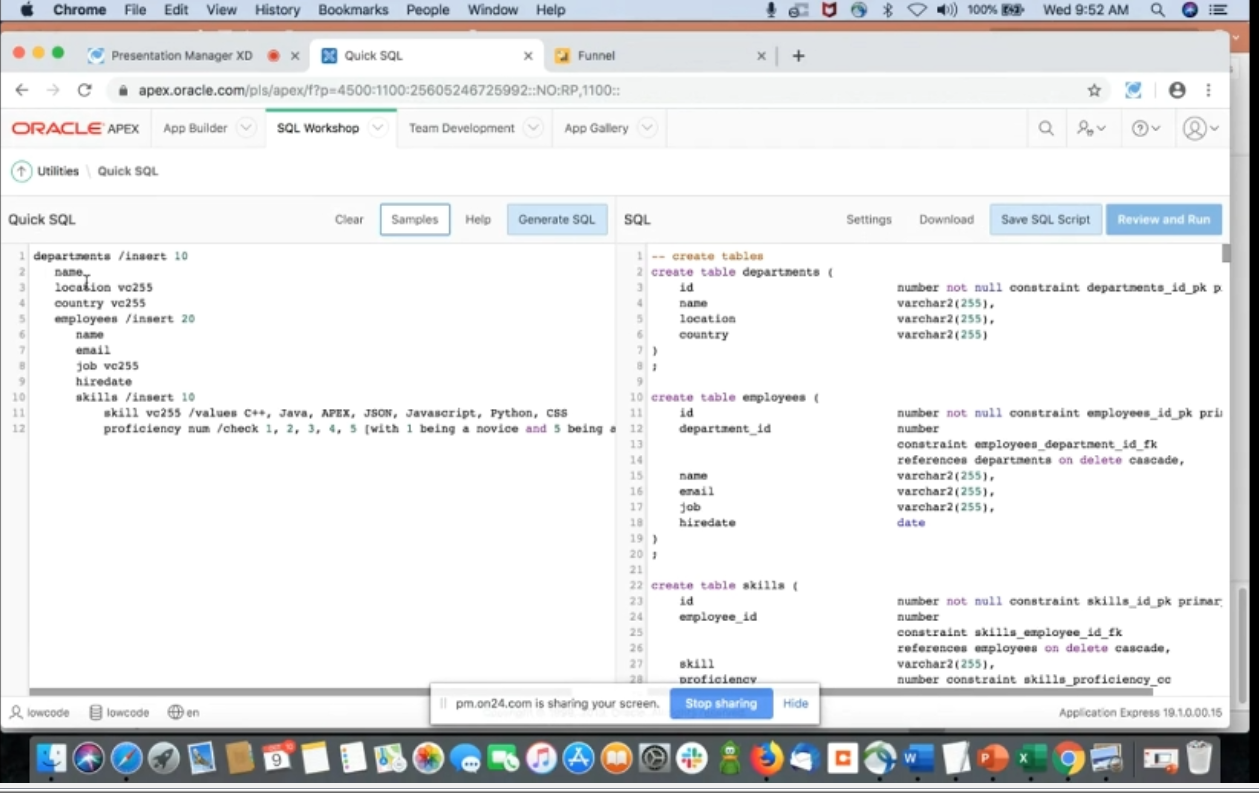
\includegraphics[scale=0.5]{figures/u}
    \caption{\textit{Sample}}
    \label{foto21}
\end{figure}
\item Pada Quick SQL kita juga bisa mengatur database yang akan kita buat pada menu Settings.
 \begin{figure}[H]
    \centering
    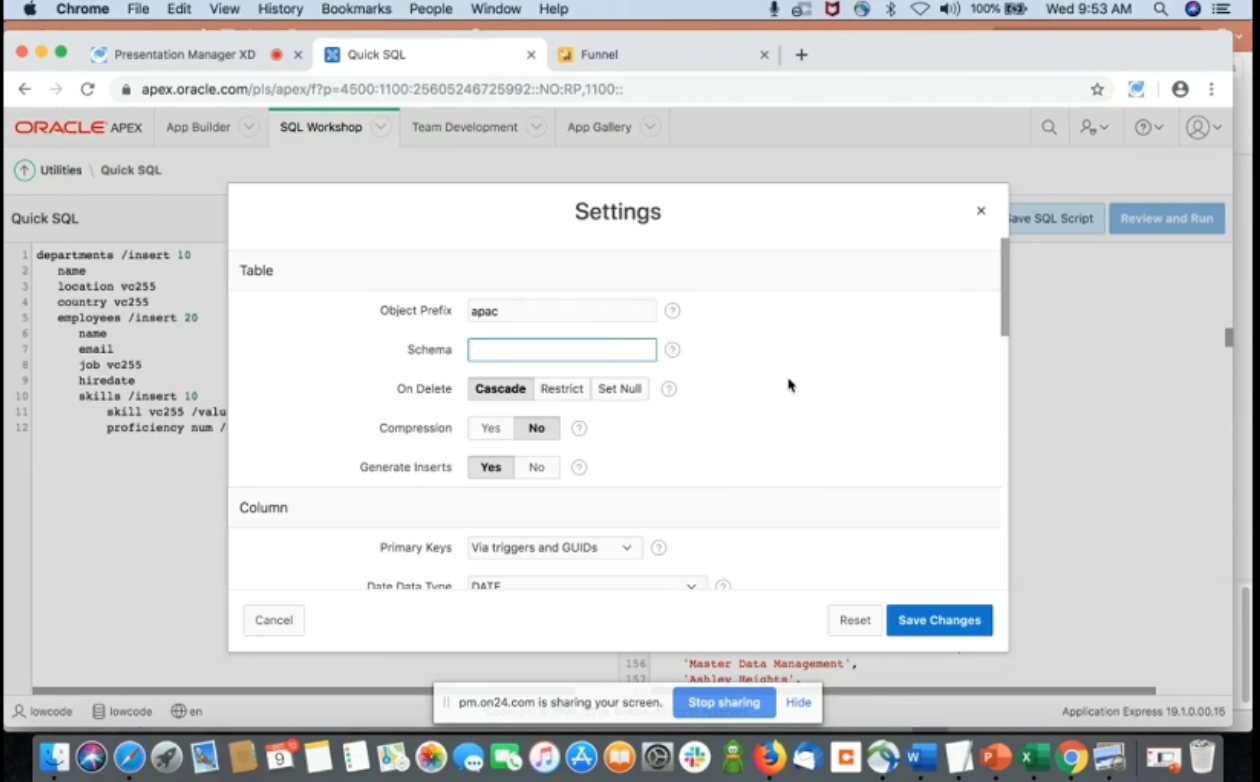
\includegraphics[scale=0.5]{figures/v}
    \caption{\textit{Settings}}
    \label{foto22}
\end{figure}
\item Menu Run Script ini berguna untuk menjalankan script sql yang telah kita buat.
 \begin{figure}[H]
    \centering
    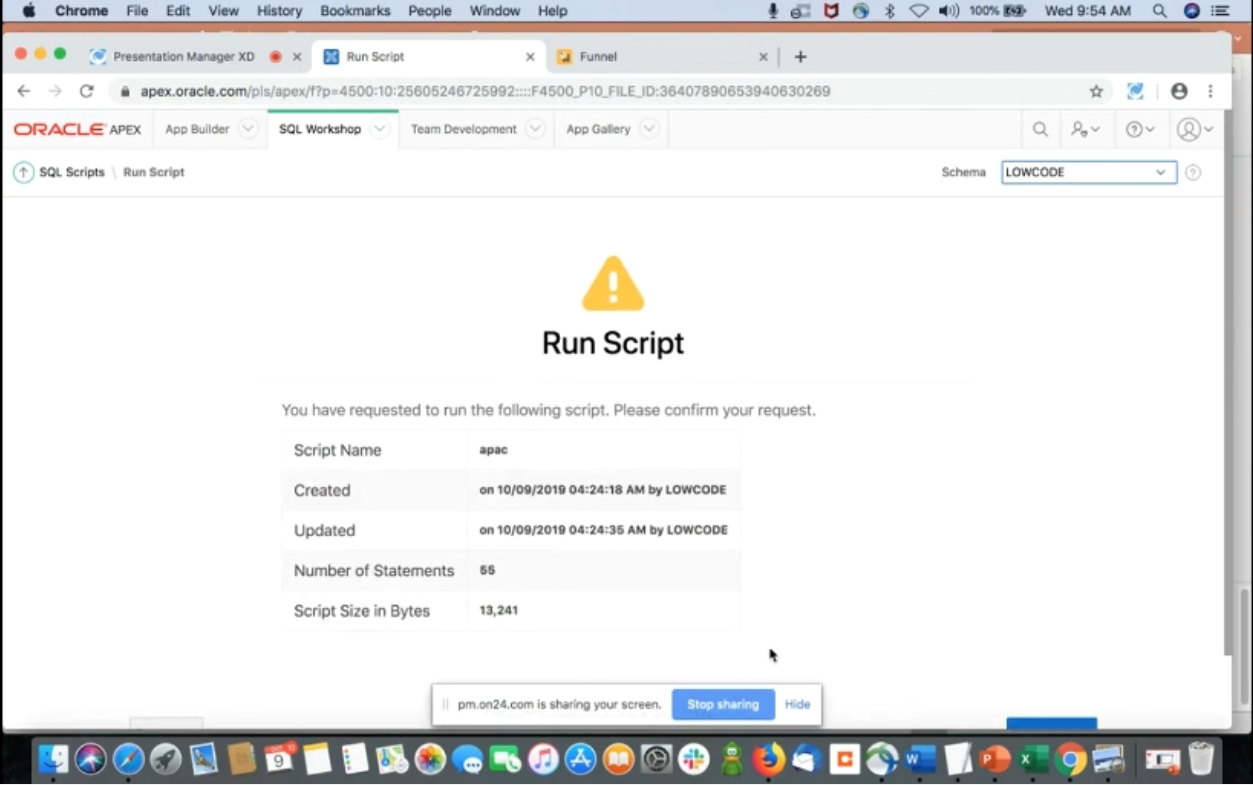
\includegraphics[scale=0.5]{figures/w}
    \caption{\textit{Run Script}}
    \label{foto23}
\end{figure}
\item  Tampilan database yang telah dijalankan.
\begin{figure}[H]
    \centering
    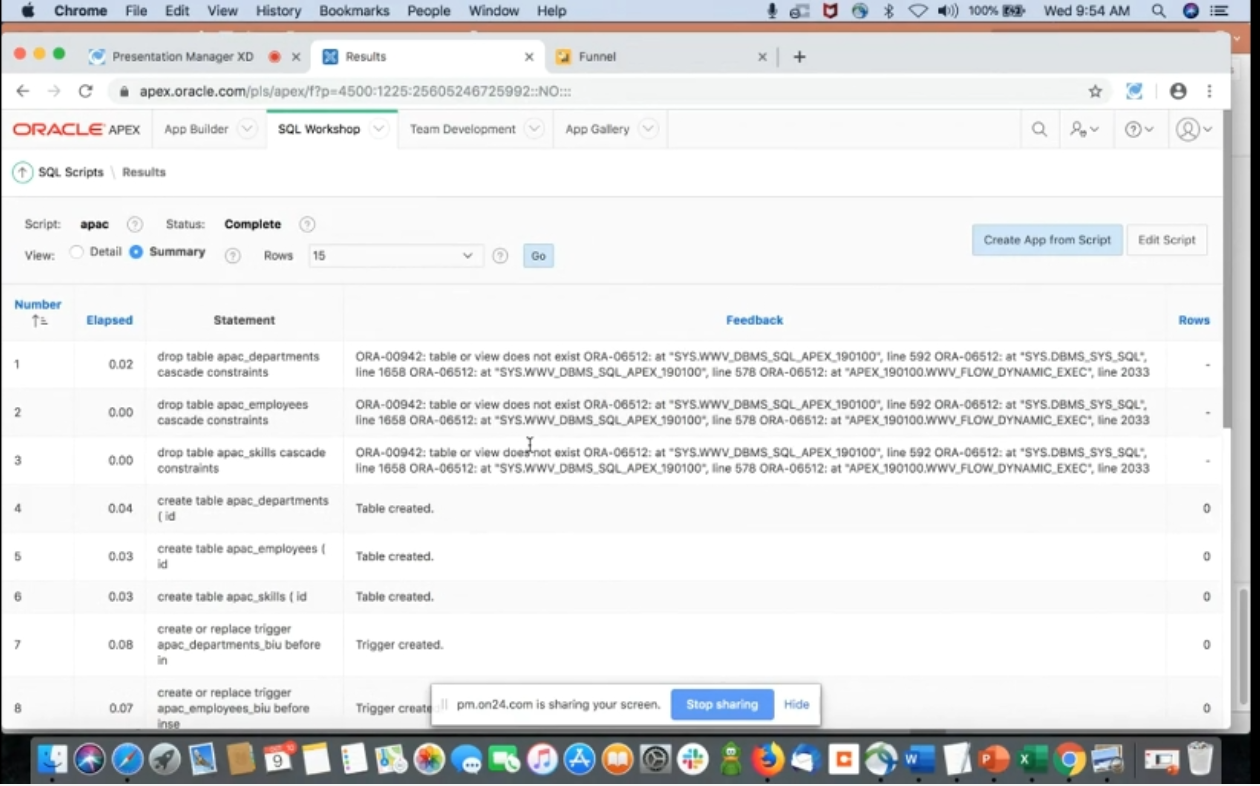
\includegraphics[scale=0.5]{figures/x}
    \caption{\textit{Run Database}}
    \label{foto24}
\end{figure}
\end{enumerate}

